\documentclass[mstat,12pt]{unswthesis}


\usepackage{array}
\usepackage{calc}
\usepackage{enumitem}
\usepackage{svg}
\usepackage{color}
\usepackage{fancyvrb}
\newcommand{\VerbBar}{|}
\newcommand{\VERB}{\Verb[commandchars=\\\{\}]}
\DefineVerbatimEnvironment{Highlighting}{Verbatim}{commandchars=\\\{\}}
% Add ',fontsize=\small' for more characters per line
\usepackage{framed}
\definecolor{shadecolor}{RGB}{248,248,248}
\newenvironment{Shaded}{\begin{snugshade}}{\end{snugshade}}
\newcommand{\AlertTok}[1]{\textcolor[rgb]{0.94,0.16,0.16}{#1}}
\newcommand{\AnnotationTok}[1]{\textcolor[rgb]{0.56,0.35,0.01}{\textbf{\textit{#1}}}}
\newcommand{\AttributeTok}[1]{\textcolor[rgb]{0.13,0.29,0.53}{#1}}
\newcommand{\BaseNTok}[1]{\textcolor[rgb]{0.00,0.00,0.81}{#1}}
\newcommand{\BuiltInTok}[1]{#1}
\newcommand{\CharTok}[1]{\textcolor[rgb]{0.31,0.60,0.02}{#1}}
\newcommand{\CommentTok}[1]{\textcolor[rgb]{0.56,0.35,0.01}{\textit{#1}}}
\newcommand{\CommentVarTok}[1]{\textcolor[rgb]{0.56,0.35,0.01}{\textbf{\textit{#1}}}}
\newcommand{\ConstantTok}[1]{\textcolor[rgb]{0.56,0.35,0.01}{#1}}
\newcommand{\ControlFlowTok}[1]{\textcolor[rgb]{0.13,0.29,0.53}{\textbf{#1}}}
\newcommand{\DataTypeTok}[1]{\textcolor[rgb]{0.13,0.29,0.53}{#1}}
\newcommand{\DecValTok}[1]{\textcolor[rgb]{0.00,0.00,0.81}{#1}}
\newcommand{\DocumentationTok}[1]{\textcolor[rgb]{0.56,0.35,0.01}{\textbf{\textit{#1}}}}
\newcommand{\ErrorTok}[1]{\textcolor[rgb]{0.64,0.00,0.00}{\textbf{#1}}}
\newcommand{\ExtensionTok}[1]{#1}
\newcommand{\FloatTok}[1]{\textcolor[rgb]{0.00,0.00,0.81}{#1}}
\newcommand{\FunctionTok}[1]{\textcolor[rgb]{0.13,0.29,0.53}{\textbf{#1}}}
\newcommand{\ImportTok}[1]{#1}
\newcommand{\InformationTok}[1]{\textcolor[rgb]{0.56,0.35,0.01}{\textbf{\textit{#1}}}}
\newcommand{\KeywordTok}[1]{\textcolor[rgb]{0.13,0.29,0.53}{\textbf{#1}}}
\newcommand{\NormalTok}[1]{#1}
\newcommand{\OperatorTok}[1]{\textcolor[rgb]{0.81,0.36,0.00}{\textbf{#1}}}
\newcommand{\OtherTok}[1]{\textcolor[rgb]{0.56,0.35,0.01}{#1}}
\newcommand{\PreprocessorTok}[1]{\textcolor[rgb]{0.56,0.35,0.01}{\textit{#1}}}
\newcommand{\RegionMarkerTok}[1]{#1}
\newcommand{\SpecialCharTok}[1]{\textcolor[rgb]{0.81,0.36,0.00}{\textbf{#1}}}
\newcommand{\SpecialStringTok}[1]{\textcolor[rgb]{0.31,0.60,0.02}{#1}}
\newcommand{\StringTok}[1]{\textcolor[rgb]{0.31,0.60,0.02}{#1}}
\newcommand{\VariableTok}[1]{\textcolor[rgb]{0.00,0.00,0.00}{#1}}
\newcommand{\VerbatimStringTok}[1]{\textcolor[rgb]{0.31,0.60,0.02}{#1}}
\newcommand{\WarningTok}[1]{\textcolor[rgb]{0.56,0.35,0.01}{\textbf{\textit{#1}}}}


\usepackage[utf8]{inputenc}
\usepackage{textcomp}
\usepackage{eurosym}



%%%%%%%%%%%%%%%%%%%%%%%%%%%%%%%%%%%%%%%%%%%%%%%%%%%%%%%%%%%%%%%%%%
% 
% OK...Now we get to some actual input.  The first part sets up
% the title etc that will appear on the front page
%
%%%%%%%%%%%%%%%%%%%%%%%%%%%%%%%%%%%%%%%%%%%%%%%%%%%%%%%%%%%%%%%%%

\title{Projet réalisé par\\[0.5cm] l'équipe TDDT du groupe de TD1 \\[3cm]Rapport
de groupe des UE \newline  Bases de données + Sciences des Données 2}

\authornameonly{ }

\author{
  \begin{tabular}{c}
  MOUTCHACHOU Lydia \\
  IBNMTAR Hazem \\
  BERETTI--PRENANT Esteban \\
  VAROL Serdar
  \end{tabular}
}

\copyrightfalse
\figurespagefalse
\tablespagefalse

%%%%%%%%%%%%%%%%%%%%%%%%%%%%%%%%%%%%%%%%%%%%%%%%%%%%%%%%%%%%%%%%%
%
%  And now the document begins
%  The \beforepreface and \afterpreface commands puts the
%  contents page etc in
%
%%%%%%%%%%%%%%%%%%%%%%%%%%%%%%%%%%%%%%%%%%%%%%%%%%%%%%%%%%%%%%%%%%


%%%%%%%%%%%%%%%%%%%%%%%%%%%%%%%%%%%%%%%%%%%%%%%%%%%%%%%%%%%%%%%%%%%%%%%
%
%  A small sample UNSW Coursework Masters thesis file.
%  Any questions to Ian Doust i.doust@unsw.edu.au and/or Gery Geenens ggeenens@unsw.edu.au
%
%%%%%%%%%%%%%%%%%%%%%%%%%%%%%%%%%%%%%%%%%%%%%%%%%%%%%%%%%%%%%%%%%%%%%%%
%
%  The first part pulls in a UNSW Thesis class file.  This one is
%  slightly nonstandard and has been set up to do a couple of
%  things automatically
%
 
%%%%%%%%%%%%%%%%%
%% Precisely one of the next four lines should be uncommented.
%% Choose the one which matches your degree, uncomment it, and comment out the other two!
%\documentclass[mfin,12pt]{unswthesis}    %%  For Master of Financial Mathematics 
%\documentclass[mmath,12pt]{unswthesis}   %%  For Master of Mathematics
%\documentclass[mstat,12pt]{unswthesis}  %%  For Master of Statistics
%%%%%%%%%%%%%%%%%



\linespread{1}
\usepackage{amsfonts}
\usepackage{amssymb}
\usepackage{amsthm}
\usepackage{latexsym,amsmath}
\usepackage{graphicx}
\usepackage{afterpage}
\usepackage[colorlinks]{hyperref}
 \hypersetup{
     colorlinks=true,
     linkcolor=blue,
     filecolor=blue,
     citecolor= black,      
     urlcolor=cyan,
     }
\usepackage{textcomp}
\usepackage{longtable}
\usepackage{booktabs}
\usepackage{float}
\let\origfigure\figure
\let\endorigfigure\endfigure
\renewenvironment{figure}[1][2] {
    \expandafter\origfigure\expandafter[H]
} {
    \endorigfigure
}
\usepackage[T1]{fontenc}
\usepackage{ragged2e}
\def\tightlist{}
\usepackage[french]{babel}

%%%%%%%%%%%%%%%%%%%%%%%%%%%%%%%%%%%%%%%%%%%%%%%%%%%%%%%%%%%%%%%%%
%
%  The following are some simple LaTeX macros to give some
%  commonly used letters in funny fonts. You may need more or less of
%  these
%
\newcommand{\R}{\mathbb{R}}
\newcommand{\Q}{\mathbb{Q}}
\newcommand{\C}{\mathbb{C}}
\newcommand{\N}{\mathbb{N}}
\newcommand{\F}{\mathbb{F}}
\newcommand{\PP}{\mathbb{P}}
\newcommand{\T}{\mathbb{T}}
\newcommand{\Z}{\mathbb{Z}}
\newcommand{\B}{\mathfrak{B}}
\newcommand{\BB}{\mathcal{B}}
\newcommand{\M}{\mathfrak{M}}
\newcommand{\X}{\mathfrak{X}}
\newcommand{\Y}{\mathfrak{Y}}
\newcommand{\CC}{\mathcal{C}}
\newcommand{\E}{\mathbb{E}}
\newcommand{\cP}{\mathcal{P}}
\newcommand{\cS}{\mathcal{S}}
\newcommand{\A}{\mathcal{A}}
\newcommand{\ZZ}{\mathcal{Z}}
%%%%%%%%%%%%%%%%%%%%%%%%%%%%%%%%%%%%%%%%%%%%%%%%%%%%%%%%%%%%%%%%%%%%%
%
% The following are much more esoteric commands that I have left in
% so that this file still processes. Use or delete as you see fit
%
\newcommand{\bv}[1]{\mbox{BV($#1$)}}
\newcommand{\comb}[2]{\left(\!\!\!\begin{array}{c}#1\\#2\end{array}\!\!\!\right)
}
\newcommand{\Lat}{{\rm Lat}}
\newcommand{\var}{\mathop{\rm var}}
\newcommand{\Pt}{{\mathcal P}}
\def\tr(#1){{\rm trace}(#1)}
\def\Exp(#1){{\mathbb E}(#1)}
\def\Exps(#1){{\mathbb E}\sparen(#1)}
\newcommand{\floor}[1]{\left\lfloor #1 \right\rfloor}
\newcommand{\ceil}[1]{\left\lceil #1 \right\rceil}
\newcommand{\hatt}[1]{\widehat #1}
\newcommand{\modeq}[3]{#1 \equiv #2 \,(\text{mod}\, #3)}
\newcommand{\rmod}{\,\mathrm{mod}\,}
\newcommand{\p}{\hphantom{+}}
\newcommand{\vect}[1]{\mbox{\boldmath $ #1 $}}
\newcommand{\reff}[2]{\ref{#1}.\ref{#2}}
\newcommand{\psum}[2]{\sum_{#1}^{#2}\!\!\!'\,\,}
\newcommand{\bin}[2]{\left( \begin{array}{@{}c@{}}
				#1 \\ #2
			\end{array}\right)	}
%
%  Macros - some of these are in plain TeX (gasp!)
%
\newcommand{\be}{($\beta$)}
\newcommand{\eqp}{\mathrel{{=}_p}}
\newcommand{\ltp}{\mathrel{{\prec}_p}}
\newcommand{\lep}{\mathrel{{\preceq}_p}}
\def\brack#1{\left \{ #1 \right \}}
\def\bul{$\bullet$\ }
\def\cl{{\rm cl}}
\let\del=\partial
\def\enditem{\par\smallskip\noindent}
\def\implies{\Rightarrow}
\def\inpr#1,#2{\t \hbox{\langle #1 , #2 \rangle} \t}
\def\ip<#1,#2>{\langle #1,#2 \rangle}
\def\lp{\ell^p}
\def\maxb#1{\max \brack{#1}}
\def\minb#1{\min \brack{#1}}
\def\mod#1{\left \vert #1 \right \vert}
\def\norm#1{\left \Vert #1 \right \Vert}
\def\paren(#1){\left( #1 \right)}
\def\qed{\hfill \hbox{$\Box$} \smallskip}
\def\sbrack#1{\Bigl \{ #1 \Bigr \} }
\def\ssbrack#1{ \{ #1 \} }
\def\smod#1{\Bigl \vert #1 \Bigr \vert}
\def\smmod#1{\bigl \vert #1 \bigr \vert}
\def\ssmod#1{\vert #1 \vert}
\def\sspmod#1{\vert\, #1 \, \vert}
\def\snorm#1{\Bigl \Vert #1 \Bigr \Vert}
\def\ssnorm#1{\Vert #1 \Vert}
\def\sparen(#1){\Bigl ( #1 \Bigr )}

\newcommand\blankpage{%
    \null
    \thispagestyle{empty}%
    \addtocounter{page}{-1}%
    \newpage}

%%%%%%%%%%%%%%%%%%%%%%%%%%%%%%%
%
% These environments allow you to get nice numbered headings
%  for your Theorems, Definitions etc.  
%
%  Environments
%
%%%%%%%%%%%%%%%%%%%%%%%%%%%%%%%

\newtheorem{theorem}{Theorem}[section]
\newtheorem{lemma}[theorem]{Lemma}
\newtheorem{proposition}[theorem]{Proposition}
\newtheorem{corollary}[theorem]{Corollary}
\newtheorem{conjecture}[theorem]{Conjecture}
\newtheorem{definition}[theorem]{Definition}
\newtheorem{example}[theorem]{Example}
\newtheorem{remark}[theorem]{Remark}
\newtheorem{question}[theorem]{Question}
\newtheorem{notation}[theorem]{Notation}
\numberwithin{equation}{section}

%%%%%%%%%%%%%%%%%%%%%%%%%%%%%%%%%%%%%%%%%%%%%%%%%%%%%%%%%%%%%%%%%%
%
%  If you've got some funny special words that LaTeX might not
% hyphenate properly, you can give it a helping hand:
%

\hyphenation{Mar-cin-kie-wicz Rade-macher}


\newlength{\cslhangindent}
\setlength{\cslhangindent}{1.5em}
\newlength{\csllabelwidth}
\setlength{\csllabelwidth}{3em}
\newenvironment{CSLReferences}[2] % #1 hanging-ident, #2 entry spacing
 {% don't indent paragraphs
  \setlength{\parindent}{0pt}
  % turn on hanging indent if param 1 is 1
  \ifodd #1 \everypar{\setlength{\hangindent}{\cslhangindent}}\ignorespaces\fi
  % set entry spacing
  \ifnum #2 > 0
  \setlength{\parskip}{#2\baselineskip}
  \fi
 }%
 {}
\usepackage{calc} % for \widthof, \maxof
\newcommand{\CSLBlock}[1]{#1\hfill\break}
\newcommand{\CSLLeftMargin}[1]{\parbox[t]{\maxof{\widthof{#1}}{\csllabelwidth}}{#1}}
\newcommand{\CSLRightInline}[1]{\parbox[t]{\linewidth}{#1}}
\newcommand{\CSLIndent}[1]{\hspace{\cslhangindent}#1}






\renewcommand{\contentsname}{Table des matières}

\renewcommand{\chaptername}{Chapitre}




\begin{document}

\beforepreface

%\afterpage{\blankpage}

% plagiarism

\prefacesection{Déclaration de non plagiat}

\textcolor{red}{À compléter avant la remise du rapport.}

\vskip 2pc \noindent Nous déclarons que ce rapport est le fruit de notre seul travail, à part lorsque cela est indiqué  explicitement. 

\vskip 2pc  \noindent Nous acceptons que la personne évaluant ce rapport puisse, pour les besoins de cette évaluation:
\begin{itemize}
\item la reproduire et en fournir une copie à un autre membre de l'université; et/ou,
\item en communiquer une copie à un service en ligne de détection de plagiat (qui pourra en retenir une copie pour les besoins d'évaluation future).
\end{itemize}

\vskip 2pc \noindent Nous certifions que nous avons lu et compris les règles ci-dessus.\vspace{24pt}

\vskip 2pc \noindent En signant cette déclaration, nous acceptons ce qui précède.
\vskip 2pc \noindent
Signature: \rule{7cm}{0.25pt} \hfill Date: \rule{4cm}{0.25pt} \\[1cm]
\vskip 1pc

%\textcolor{red}{Mettre à jour la date.}

{\bigskip\bigskip\bigskip\noindent} \today
%\afterpage{\blankpage}

% Acknowledgements are optional


\prefacesection{Remerciements}

\textcolor{red}{À compléter avant la remise du rapport.}

{\bigskip}Nos plus sincères remerciements vont à notre encadrant
pédagogique pour les conseils avisés sur notre travail.\\[1cm] Nous
remercions aussi \ldots{}\\[1cm] 

{\bigskip\bigskip\bigskip\noindent} \today

%\afterpage{\blankpage}

% Abstract

\prefacesection{Résumé}

Notre projet vise à analyser les performances financières des
entreprises françaises entre 2018 et 2022 à partir des données du
Registre National du Commerce et des Sociétés (RNCS). Nous cherchons à
comprendre quels sont les facteurs qui influencent la rentabilité des
entreprises et comment ces dernières évoluent en fonction de leur
secteur d'activité. Plus précisément, nous allons : - Comparer les
performances des entreprises selon leur chiffre d'affaires et leur
rentabilité. - Étudier l'impact de la fiscalité sur la profitabilité des
entreprises. - Analyser l'évolution des ventes, des stocks et des taxes
pour identifier des tendances économiques.

%\afterpage{\blankpage}


\afterpreface





%%%%%%%%%%%%%%%%%%%%%%%%%%%%%%%%%%%%%%%%%%%%%%%%%%%%%%%%%%%%%%%%%%
%
% Now we can start on the first chapter
% Within chapters we have sections, subsections and so forth
%
%%%%%%%%%%%%%%%%%%%%%%%%%%%%%%%%%%%%%%%%%%%%%%%%%%%%%%%%%%%%%%%%%%



%%%%%%%%%%%%%%%%%%%%%%%%%%%%%%%%%%%%%

%\afterpage{\blankpage}


\chapter{Introduction}\label{introduction}

\section{Présentation du projet}\label{pruxe9sentation-du-projet}

Les données financières des entreprises jouent un rôle crucial dans la
compréhension de leur santé économique. Ce projet se concentre sur
l'analyse des performances financières des entreprises françaises entre
2018 et 2022, en utilisant les données fournies par le Registre National
du Commerce et des Sociétés (RNCS).

\bigskip

\begin{itemize}[label=$\circ$]
    \item \textbf{Comparer les performances des entreprises selon leur chiffre d'affaires et leur rentabilité.}
    \item \textbf{Étudier l’impact de la fiscalité sur la profitabilité des entreprises.}
    \item \textbf{Analyser l’évolution des ventes, des stocks et des taxes pour identifier des tendances économiques.}
\end{itemize}

\medskip

\section{Responsabilités et composition de
l'équipe}\label{responsabilituxe9s-et-composition-de-luxe9quipe}

\medskip

MOUTCHACHOU Lydia : Étudiant n°22212656

IBNMTAR Hazem : Étudiant n°22309227

BERETTI--PRENANT Esteban : Étudiant n°22208752

VAROL Serdar : Étudiant n°22009668

\bigskip

\section{Objectifs et questions de
recherche}\label{objectifs-et-questions-de-recherche}

Notre projet vise à analyser les performances financières des
entreprises françaises entre 2018 et 2022. Pour ce faire, nous allons
examiner plusieurs facteurs qui pourraient influencer la rentabilité des
entreprises. Les questions spécifiques que nous allons aborder sont les
suivantes :

\medskip

\textbf{Comparaison de la rentabilité par rapport au chiffre d'affaires
:}

\begin{enumerate}
\def\labelenumi{\alph{enumi}.}
\item
  Comment la rentabilité varie-t-elle en fonction de la taille de
  l'entreprise ?
\item
  Y a-t-il une différence notable entre les entreprises qui ont recours
  au refinancement et celles qui n'en ont pas besoin ?
\end{enumerate}

\textbf{Comparaison de la rentabilité par rapport au chiffre}

\begin{enumerate}
\def\labelenumi{\alph{enumi}.}
\item
  La rentabilité des entreprises diffère-t-elle selon la ville où elles
  sont implantées ?
\item
  Les entreprises qui exportent leurs produits ou services sont-elles
  plus rentables que celles qui opèrent uniquement sur le marché
  national ?
\end{enumerate}

\textbf{Impact fiscal et sectoriel :}

\begin{enumerate}
\def\labelenumi{\alph{enumi}.}
\item
  Quel est l'impact des taxes sur la rentabilité des entreprises ?
\item
  Comment la rentabilité varie-t-elle selon le secteur d'activité des
  entreprises ?
\end{enumerate}

\textbf{Évolution temporelle :}

\begin{enumerate}
\def\labelenumi{\alph{enumi}.}
\item
  Comment la rentabilité des entreprises a-t-elle évolué entre 2012 et
  2016 ?
\item
  Peut-on identifier des tendances spécifiques ou des périodes de
  croissance/déclin dans les performances financières des entreprises ?
\end{enumerate}

\medskip

En répondant à ces questions, nous espérons identifier les principaux
facteurs influençant la rentabilité des entreprises françaises et
fournir des insights précieux pour les décideurs économiques et les
gestionnaires d'entreprises.

\chapter{Base de données}\label{base-de-donnuxe9es}

\section{Provenance des données}\label{provenance-des-donnuxe9es}

Les données utilisées dans ce projet proviennent du jeu de données
Kaggle : \medskip

\begin{itemize}[label=$\circ$]
  \item \textnormal{\textbf{Profit and loss \- Ontology.csv :} Contient les comptes de résultat de 100 000 entreprises françaises, avec des informations détaillées sur les revenus, les dépenses et les bénéfices.}
  
  \item \textnormal{\textbf{APE\_Fusion.csv :} Utilise le code APE pour classer les entreprises selon leur secteur d’activité, permettant des comparaisons sectorielles précises.}

  \item \textnormal{\textbf{Data\_Kaggle.csv :} Fournit des données globales sur les entreprises, incluant les ventes, les stocks et les taxes, permettant d'analyser l’évolution des performances financières sur plusieurs années.}
\end{itemize}

\medskip

\textit{Lien vers les données :}
\href{https://www.kaggle.com/datasets/briaclg/financial-data-of-french-compagnies/data?select=Profit+and+loss+-+Onthology.csv}{Kaggle Dataset}

\section{Descriptif des tables}\label{descriptif-des-tables}

\bigskip

\subsection{Table 1: APE\_Fusion.csv}\label{table-1-ape_fusion.csv}

\begin{table}[H]
\centering
\scriptsize
\begin{tabular}{|p{3.2cm}|p{1.2cm}|p{7.5cm}|p{2.5cm}|}
\hline
\textbf{Nom colonne} & \textbf{Type} & \textbf{Signification} & \textbf{Caractéristique} \\
\hline
Unname d: 0 & int & Index ou identifiant de ligne (peut être ignoré dans l'analyse) & \\
\hline
ape & object & Code APE complet de l'activité principale de l'entreprise & Clé primaire \\
\hline
ape\_name & object & Nom ou description de l'activité correspondant au code APE & \\
\hline
ape\_len & int & Longueur du code APE, indiquant le nombre de caractères qu'il contient & \\
\hline
ape\_cat0 & int & Premier niveau du code APE (division), composé des 2 premiers chiffres & \\
\hline
ape\_cat1 & float & Deuxième niveau du code APE (groupe), composé des 3 premiers chiffres & \\
\hline
ape\_cat2 & float & Troisième niveau du code APE (classe), composé des 4 premiers chiffres & \\
\hline
ape\_cat3 & object & Dernier niveau du code APE (sous-classe) & \\
\hline
Libellé & object & Description du secteur d'activité auquel appartient le code APE & \\
\hline
Code & object & Code alphabétique supplémentaire associé au secteur d'activité & \\
\hline
\end{tabular}
\footnotesize
\label{tab:ape_description}
\end{table}

\subsection{Table 2 : Profit and loss -
Ontology.csv}\label{table-2-profit-and-loss---ontology.csv}

\begin{table}[H]
\centering
\scriptsize
\begin{tabular}{|p{4cm}|p{2cm}|p{9cm}|}
\hline
\textbf{Nom colonne} & \textbf{Type} & \textbf{Signification} \\
\hline
Columns\_(FR/EN) & varchar & Colonnes des états financiers en français et en anglais \\
\hline
Description (FR) & varchar & Explication de ce que chaque colonne représente \\
\hline
Liasse (Id) & int & Identifiant unique des colonnes dans la base INPI \\
\hline
Calcul & varchar & Méthode de calcul pour certaines valeurs dans les colonnes \\
\hline
\end{tabular}
\normalsize
\end{table}

\subsection{Table 3 : Data\_Kaggle.csv}\label{table-3-data_kaggle.csv}

\scriptsize
\begin{longtable}{|p{0.7cm}|p{12cm}|p{1.5cm}|}
\hline
\textbf{N\textdegree} & \textbf{Variable} & \textbf{Code} \\
\hline \endfirsthead
\hline \textbf{N\textdegree} & \textbf{Variable Nome} & \textbf{Nome de Colon} \\ \hline \endhead
1 & year & B \\
2 & Autres imp\^ots, taxes et versements assimil\'es & C \\
3 & Ventes de marchandises & D \\
4 & Production vendue biens & E \\
5 & Production vendue services & F \\
6 & Chiffres d\'affaires nets & G \\
7 & Production stock\'ee & H \\
8 & Production immobilis\'ee & I \\
9 & Subventions d\'exploitation & J \\
10 & Reprises sur amortissements et provisions, transfert de charges & K \\
11 & Autres produits & L \\
12 & Total des produits d\'exploitation & M \\
13 & Achats de marchandises (y compris droits de douane) & N \\
14 & Variation de stock (marchandises) & O \\
15 & Achats de mati\`eres premi\`eres et autres approvisionnements & P \\
16 & Variation de stock (mati\`eres premi\`eres et approvisionnements) & Q \\
17 & Autres achats et charges externes & R \\
18 & Imp\^ots, taxes et versements assimil\'es & S \\
19 & Salaires et traitements & T \\
20 & Charges sociales & U \\
21 & Autres charges & V \\
22 & Total des charges d\'exploitation & W \\
23 & R\'esultat d'exploitation & X \\
24 & B\'en\'efice attribu\'e ou perte transf\'er\'ee & Y \\
25 & Perte support\'ee ou b\'en\'efice transf\'er\'e & Z \\
26 & Produits financiers de participations & AA \\
27 & Produits des autres valeurs mobili\`eres et cr\'eances de l\'actif immobilis\'e & AB \\
28 & Autres int\'er\^ets et produits assimil\'es & AC \\
29 & Reprises sur provisions et transferts de charges financier & AD \\
30 & Diff\'erences positives de change & AE \\
31 & Produits nets sur cessions de valeurs mobili\`eres de placement & AF \\
32 & Total des produits financiers & AG \\
33 & Dotations financi\`eres sur amortissements et provisions & AH \\
34 & Int\'er\^ets et charges assimil\'ees & AI \\
35 & Diff\'erences n\'egatives de change & AJ \\
36 & Charges nettes sur cessions de valeurs mobili\`eres de placement & AK \\
37 & Total des charges financi\`eres & AL \\
38 & R\'esultat financier & AM \\
39 & R\'esultat en cours avant imp\^ots & AN \\
40 & Produits exceptionnels sur op\'erations de gestion & AO \\
41 & Produits exceptionnels sur op\'erations en capital & AP \\
42 & Reprises sur provisions et transferts de charges exceptionnel & AQ \\
43 & Total des produits exceptionnels & AR \\
44 & Charges exceptionnelles sur op\'erations de gestion & AS \\
45 & Charges exceptionnelles sur op\'erations en capital & AT \\
46 & Dotations exceptionnelles aux amortissements et provisions & AU \\
47 & Total des charges exceptionnelles & AV \\
48 & R\'esultat exceptionnel & AW \\
49 & Participation des salari\'es aux r\'esultats de l\'entreprise & AX \\
50 & Imp\^ots sur les b\'en\'efices & AY \\
51 & Total des produits & AZ \\
52 & Total des charges & BA \\
53 & B\'en\'efices ou perte (Total des produits - Total des charges) & BB \\
54 & Imp\^ots diff\'er\'es (compte de r\'esultat) & BC \\
55 & R\'esultat net des soci\'et\'es mises en \'equivalence & BD \\
56 & R\'esultat net des entreprises int\'egr\'ees & BE \\
57 & R\'esultat Groupe (R\'esultat net consolid\'e) & BF \\
58 & Part des int\'er\^ets minoritaires (R\'esultat hors groupe) & BG \\
59 & R\'esultat net part du groupe (part de la soci\'et\'e m\`ere) & BH \\
60 & R\'emun\'eration d\'interm\'ediaires et honoraires (hors r\'etrocessions) & BI \\
61 & Location, charges locatives et de copropri\'et\'e & BJ \\
62 & Effectif moyen du personnel & BK \\
63 & Sous-traitance & BL \\
64 & Personnel ext\'erieur \`a l\'entreprise & BM \\
65 & R\'etrocessions d\'honoraires, commissions et courtages & BN \\
66 & Taxe professionnelle & BO \\
67 & Montant de la TVA. collect\'ee & BP \\
\hline
\end{longtable}
\normalsize
\scriptsize
\begin{longtable}{|p{0.7cm}|p{12cm}|p{1.5cm}|}
\hline
\textbf{N\textdegree} & \textbf{Variable} & \textbf{Code} \\
\hline \endfirsthead
\hline \textbf{N\textdegree} & \textbf{Variable Nome} & \textbf{Nome de Colon} \\ \hline \endhead
68 & Total TVA. d\'eductible sur biens et services & BQ \\
69 & Dividendes & BR \\
70 & siren & BS \\
\hline
\end{longtable}
\normalsize

\newpage

\section{Modèles MCD et MOD}\label{moduxe8les-mcd-et-mod}

\begin{itemize}
\tightlist
\item
  Pour le MCD, inclure une image réalisée avec le logiciel Mocodo
  \href{https://www.mocodo.net/?mcd=eNqNksFu2zAMhu96Ch0dQAOW7Zab67ZK2zTL4ixtcjEUh14FOJKhyFm3N_J9b-AX62_HaOMEAwb4Ay1SIvlLjMvNQRmvrRnxWDsywe3DQPD43R296MwRCw9Wu7AgMRzy2Ka6rnxdieGUwyfJsKMZNUsBpmrX2kj5z50ddvZLZ7-Kid5QniNNZLfEMoXyTTWUC7OM3EWpLpggiq2j0BgixhyldLClQ8uC945wnPkQ0u1_D49auYJfk7E7fdwjeNNKYfde5WJhf8GBZtlM_SYXvSj380w_b7tq_Ena3lNX5KzT05u9DcE1kOAePIIp-AZm4DuYM3bzWljnyc2c3ZbaX9btAv3CSzJbR01Il_97pi-g12sMFuAHWIIn8AxWYC24_PNp9cxGDN9Z5pMsEiLlA5gAiJUQKyFWQuwYlzG-AhHApaxvBF8h-WrNIrsrvNroXHtqH79Z05z2Ze5VTxm_nA1xoVX866VO0_bEz-uqdfqEXovcavxhQgIpe7FMG2VSTS6Qy4H48Ktm6hK9K-q_fh_Ip7OEKRVNNkN5ML5DbGExcUlxbHkfjCcDcXSlbc_wPGLXVV2Zusp0SklBGI5gPB2wN-SeTJ4=}{https://www.moc\\odo.net}
  telle que celle visible sur la Figure\(~\)\ref{MCD} ci-dessous :
\end{itemize}

\begin{figure}
\centering
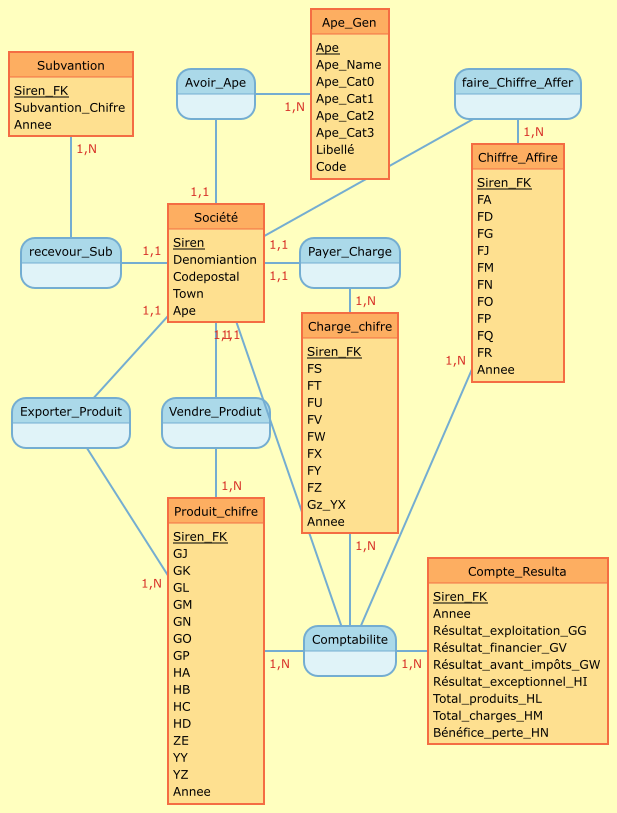
\includegraphics[width=8cm,height=10cm]{image_sql/MCD.png}
\caption{MCD}\label{MCD}
\end{figure}

\begin{itemize}
\tightlist
\item
  Pour le MOD, inclure les images réalisée avec le logiciel MySQL, telle
  que celles visible sur la Figure ci-dessous :
\end{itemize}

\begin{figure}
\centering
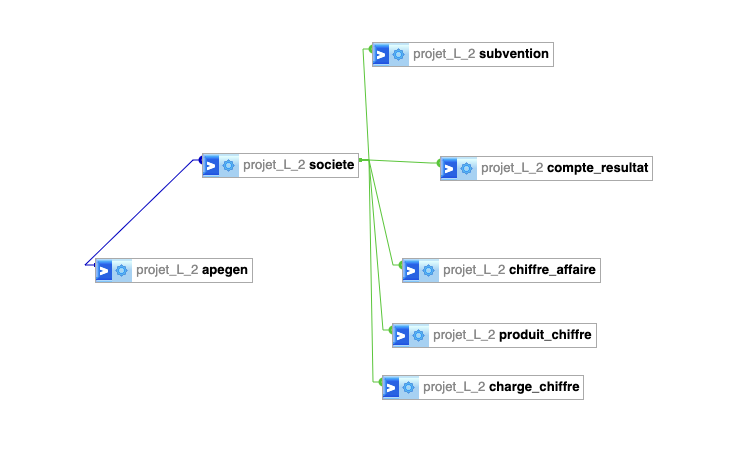
\includegraphics[width=10cm,height=5cm]{image_sql/mssql_1.png}
\caption{MOD}\label{M0D}
\end{figure}

\begin{figure}
\centering
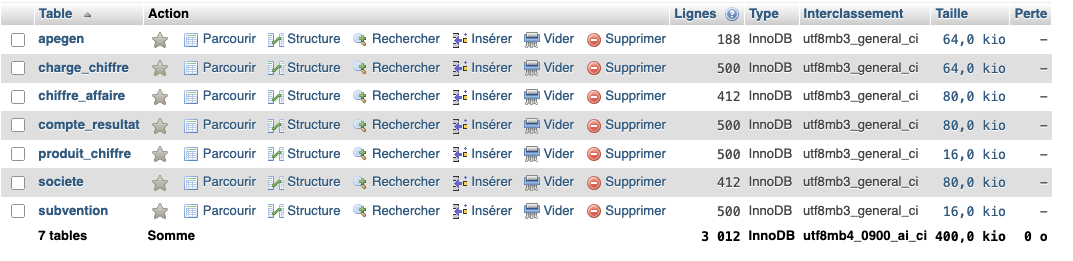
\includegraphics[width=15cm,height=5cm]{image_sql/mcd_totat.png}
\caption{MOD Table Total}\label{MOD_total}
\end{figure}

\begin{figure}
\centering
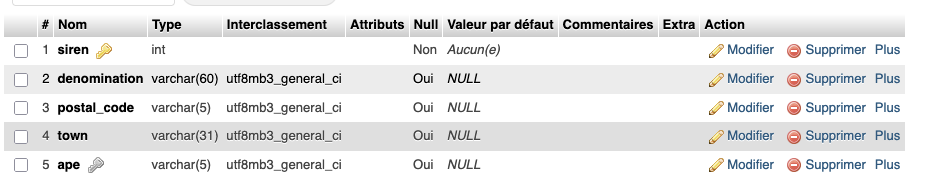
\includegraphics[width=15cm,height=5cm]{image_sql/societe.png}
\caption{Societe Table}\label{Societe}
\end{figure}

\begin{figure}
\centering
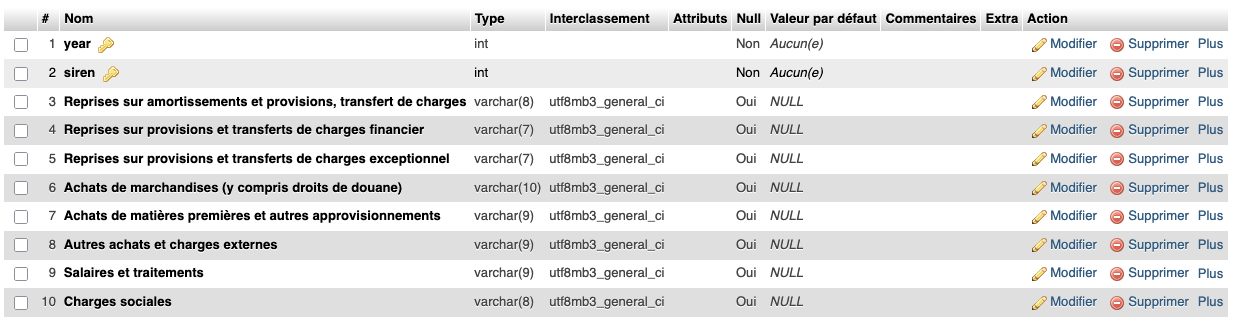
\includegraphics[width=15cm,height=5cm]{image_sql/charge_chiffre.png}
\caption{Charge Chiffre}\label{charge_chiffre}
\end{figure}

\begin{figure}
\centering
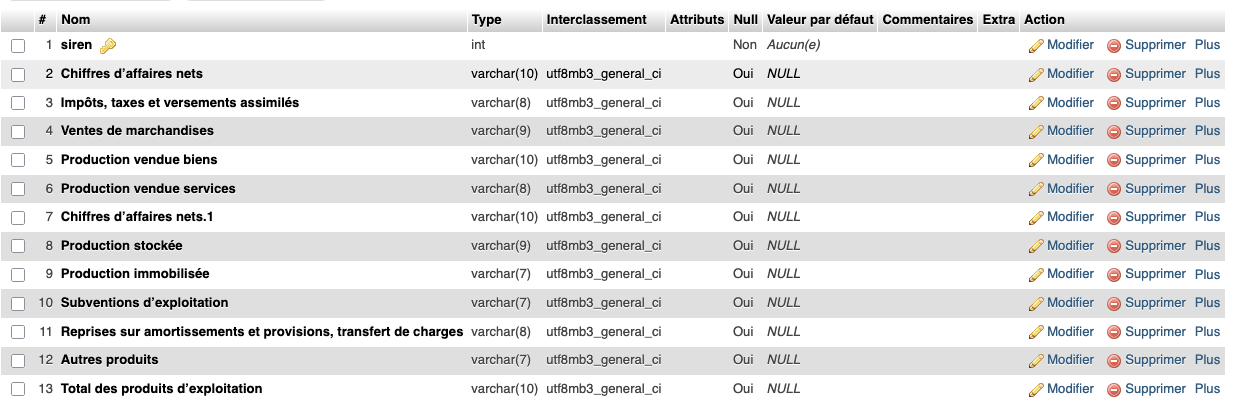
\includegraphics[width=15cm,height=5cm]{image_sql/chiffre_affaire.png}
\caption{Chiffre affaire}\label{Chiffre_affaire}
\end{figure}

\begin{figure}
\centering
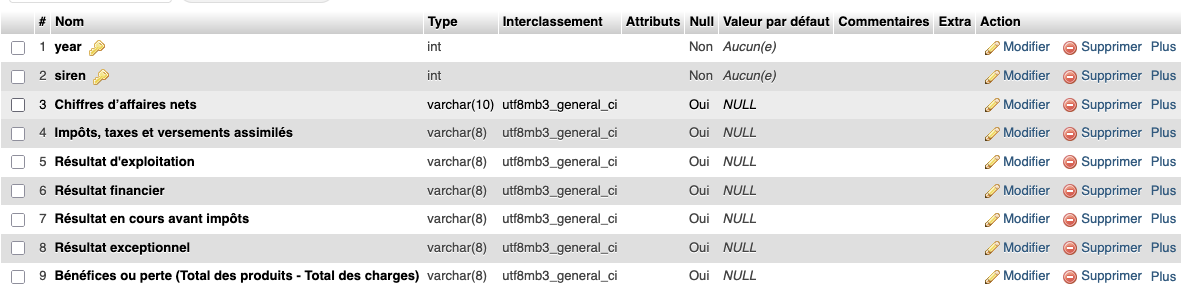
\includegraphics[width=15cm,height=5cm]{image_sql/compte_resulta.png}
\caption{Compte de Résultat}\label{compte_resulta}
\end{figure}

\begin{figure}
\centering
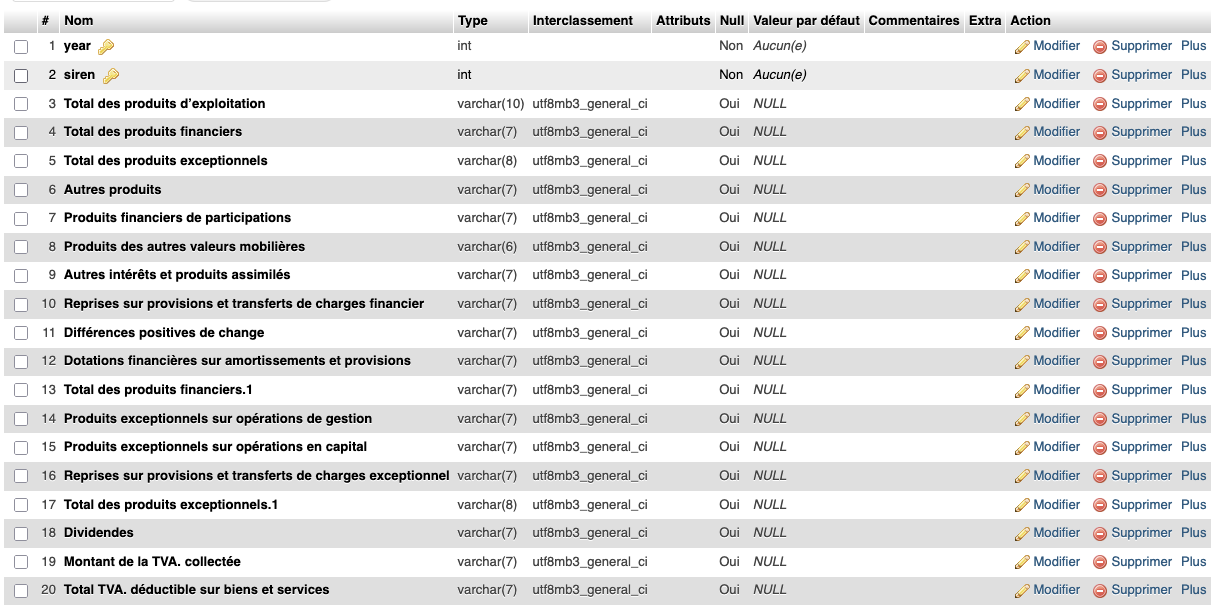
\includegraphics[width=15cm,height=5cm]{image_sql/produit_chiffre.png}
\caption{Produit Chiffre}\label{produit_chiffre}
\end{figure}

\begin{figure}
\centering
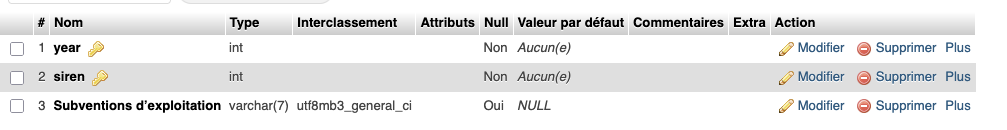
\includegraphics[width=15cm,height=3cm]{image_sql/subvention.png}
\caption{Subvention}\label{subvention}
\end{figure}

\newpage

\bigskip

\section{Import des données}\label{import-des-donnuxe9es}

\bigskip

Dans un premier temps, les données ont été chargées dans R à l'aide de
la fonction \(read\_csv()\). Ensuite, afin de faciliter l'importation de
ces données dans phpMyAdmin, nous avons procédé à un découpage (slicing)
de la base initiale en sept tables distinctes, chacune regroupant les
variables pertinentes pour son thème spécifique.

\medskip

Par exemple, pour la table \emph{``société''}, nous avons conservé
uniquement les colonnes suivantes : \emph{``siren'', ``denomination'',
``postal\_code'', ``town'' et ``ape''.}

Ce processus a été appliqué à chaque table en sélectionnant les
attributs nécessaires, puis nous avons limité chaque sous-table à ses
300 premières lignes afin de simplifier les tests d'importation.

\medskip

Enfin, les tables ont été exportées au format CSV à l'aide de la
fonction \(write\_csv\).

\medskip

Dans un premier temps, nous avions extrait les \textbf{300} premières
lignes de la base de données globale. Toutefois, afin d'obtenir un
échantillon plus équilibré et représentatif dans le temps, nous avons
modifié notre approche : nous avons sélectionné les \textbf{100
premières} lignes pour chaque année, de \textbf{2012} à \textbf{2016.}

\medskip

Pour cela, nous avons utilisé la bibliothèque sqldf dans R, qui permet
d'exécuter des requêtes SQL directement sur des data frames. Par
exemple, pour extraire les données de l'année 2012, nous avons utilisé
la requête suivante :

\begin{Shaded}
\begin{Highlighting}[]
\NormalTok{annee\_2012 }\OtherTok{\textless{}{-}} \FunctionTok{sqldf}\NormalTok{(}\StringTok{"SELECT * FROM data\_kaggle WHERE year = 2012"}\NormalTok{)}
\end{Highlighting}
\end{Shaded}

\medskip

Cette commande retourne toutes les colonnes de la base data\_kaggle pour
les lignes dont l'année est égale à 2012.

\medskip

Nous avons ensuite appliqué la même méthode pour chaque année
(\textbf{2013 à 2016}), puis extrait les 100 premières lignes de chaque
sous-ensemble. Enfin, nous avons combiné ces sous-ensembles afin
d'obtenir une table finale regroupant \textbf{500 lignes} (100 par
année). Cette nouvelle table est ainsi mieux structurée pour les futures
analyses et pourra être importée dans phpMyAdmin pour les étapes
suivantes de notre projet.

\medskip

Lors de l'importation de données sur phpMyAdmin, on a rencontré un petit
problème : la colonne était trop longue pour être insérée dans la table.
Du coup, on a modifié simplement le nom de la colonne. Elle était : «
Produits des autres valeurs mobilières et créances de l'actif immobilisé
» et on l'a changée pour : « Produits des autres valeurs mobilières ».

\medskip

Cette commande retourne toutes les colonnes de la base data\_kaggle pour
les lignes dont l'année est \textbf{égale à 2012}. Nous avons ensuite
appliqué la même méthode pour chaque année (2013 à 2016), puis extrait
\textbf{les 100 premières lignes} de chaque sous-ensemble. Enfin, nous
avons combiné ces sous-ensembles afin d'obtenir une \textbf{table finale
regroupant 500 lignes (100 par année)}. Cette nouvelle table est ainsi
mieux structurée pour les futures analyses et pourra être
\textbf{importée dans phpMyAdmin} pour les étapes suivantes de notre
projet.

\newpage

\newpage

\section{Requêtes réalisées}\label{requuxeates-ruxe9alisuxe9es}

Pour chaque requête, l'exprimer en langage naturel puis en SQL. Puis
donner le résultat obtenu (ou un extrait) et expliquer ce résultat.

L'objectif est de varier le type de requêtes et de répondre à votre
problématique initiale.

\begin{enumerate}
\def\labelenumi{\arabic{enumi})}
\tightlist
\item
  Pour comperer et trouver selon leur code postal
\end{enumerate}

\begin{Shaded}
\begin{Highlighting}[]

\KeywordTok{SELECT} 
    \KeywordTok{LEFT}\NormalTok{(postal\_code, }\DecValTok{2}\NormalTok{) }\KeywordTok{AS}\NormalTok{ departement,}
    \FunctionTok{COUNT}\NormalTok{(}\OperatorTok{*}\NormalTok{) }\KeywordTok{AS}\NormalTok{ nombre\_entreprises}
\KeywordTok{FROM} 
\NormalTok{    societe}
\KeywordTok{WHERE} 
\NormalTok{    postal\_code }\KeywordTok{IS} \KeywordTok{NOT} \KeywordTok{NULL}
\KeywordTok{GROUP} \KeywordTok{BY} 
\NormalTok{    departement}
\KeywordTok{ORDER} \KeywordTok{BY} 
\NormalTok{    nombre\_entreprises }\KeywordTok{DESC}\NormalTok{;}
\end{Highlighting}
\end{Shaded}

\begin{figure}
\centering
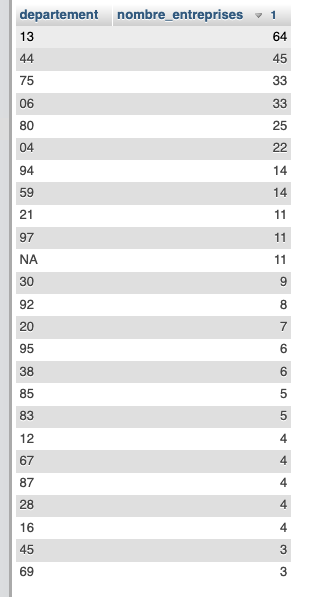
\includegraphics[width=5cm,height=10cm]{image_sql/sql_1_Serdar.png}
\caption{Code postal}
\end{figure}

\newpage

\begin{Shaded}
\begin{Highlighting}[]
\KeywordTok{SELECT} 
\NormalTok{    s.siren,}
\NormalTok{    s.denomination,}
\NormalTok{    s.postal\_code,}
\NormalTok{    cr.\textasciigrave{}Chiffres d’affaires nets\textasciigrave{} }\KeywordTok{AS}\NormalTok{ chiffre\_affaires\_net}
\KeywordTok{FROM} 
\NormalTok{    societe s}
\KeywordTok{JOIN} 
\NormalTok{    compte\_resultat cr }\KeywordTok{ON}\NormalTok{ s.siren }\OperatorTok{=}\NormalTok{ cr.siren}
\KeywordTok{WHERE} 
    \KeywordTok{LEFT}\NormalTok{(s.postal\_code, }\DecValTok{2}\NormalTok{) }\OperatorTok{=} \StringTok{\textquotesingle{}44\textquotesingle{}}\NormalTok{;}
\end{Highlighting}
\end{Shaded}

\begin{figure}
\centering
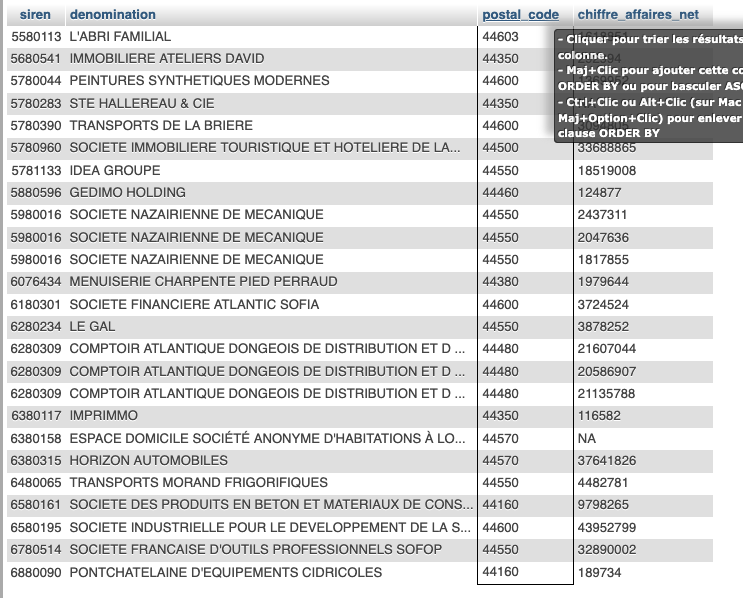
\includegraphics[width=10cm,height=10cm]{image_sql/sql_2_serdar.png}
\caption{Code postal}
\end{figure}

\chapter{Matériel et Méthodes}\label{matuxe9riel-et-muxe9thodes}

\section{Logiciels}\label{logiciels}

Nous avons utilisé ces logiciels lors de la réalisation de notre projet
:

\begin{itemize}
\tightlist
\item
  Pretraitment : Libre Office
\item
  Stocker Base Donnée : Mysql /MAMP
\item
  Traitment statistique et ecrit: R
\item
  Correction/ replacement: Regex
\item
  Version control : GitHUB
\item
  L'IA : OpenAI et MISTRAL
\end{itemize}

\bigskip

Voici lien de github notre projet :
\href{https://github.com/serdarvarl/Project_DataBase_FR.git}{TDDT github}

\section{Modélisation statistique}\label{moduxe9lisation-statistique}

\url{http://biostatisticien.eu/springeR/livreR.pdf}

\chapter{Analyse et Résultats}\label{analyse-et-ruxe9sultats}

\section{\texorpdfstring{\textbf{Comparer les catégories d'entreprises
en fonction des Chiffres d'affaires
nets}}{Comparer les catégories d'entreprises en fonction des Chiffres d'affaires nets}}\label{comparer-les-catuxe9gories-dentreprises-en-fonction-des-chiffres-daffaires-nets}

\bigskip

\textbf{Variables :} Chiffres d'affaires nets , catégories (Effectif
moyen du personnel)

\subsubsection{Les catégories d'entreprises
:}\label{les-catuxe9gories-dentreprises}

\bigskip
\scriptsize
\begin{quote}
\textit{L’article 51 de la loi n°2008-776 du 4 août 2008 de modernisation de l’économie (\textbf{LME}) détermine, pour les besoins de l’analyse statistique, un classement des entreprises en quatre catégories : les microentreprises, les petites et moyennes entreprises (\textbf{PME}), les entreprises de taille intermédiaire (\textbf{ETI}) et les grandes entreprises.\\ \\Le décret n° 2008-1354 du 18 décembre 2008 précise les critères permettant de déterminer l’appartenance à une catégorie d'entreprises.}
\end{quote}
\normalsize

\begin{itemize}[label=$\circ$]
  \item \textnormal{ \textbf{La microentreprise} est une entreprise dont l'effectif est inférieur à 10 personnes et dont le chiffre d'affaires ou le total du bilan annuel n'excède pas 2 millions d'euros}
\item \textnormal{ \textbf{la PME} est une entreprise dont l’effectif est inférieur à 250 personnes
et dont le chiffre d’affaires annuel n'excède pas 50 millions d'euros ou
dont le total de bilan n'excède pas 43 millions d'euros }
\item \textnormal{\textbf{L'ETI}, entreprise de taille intermédiaire, est une entreprise qui n'appartient pas à la catégorie des PME, dont l’effectif est inférieur à 5000 personnes et dont le chiffre d'affaires annuel n'excède pas 1 500 millions d'euros ou dont le total de bilan n'excède pas 2 000 millions d'euros}
\item \textnormal{\textbf{La grande entreprise} est une entreprise qui ne peut pas être classée
dans les catégories précédentes}
\end{itemize}

\newpage

\subsection{Test Statistique : ANOVA}\label{test-statistique-anova}

\medskip

\subsubsection{\texorpdfstring{\textbf{2012}}{2012}}\label{section}

\medskip

\begin{verbatim}
##              Df    Sum Sq   Mean Sq F value Pr(>F)    
## categorie     2 3.406e+16 1.703e+16   817.9 <2e-16 ***
## Residuals   204 4.248e+15 2.082e+13                   
## ---
## Signif. codes:  0 '***' 0.001 '**' 0.01 '*' 0.05 '.' 0.1 ' ' 1
\end{verbatim}

\begin{itemize}
\item
  Détail du test :
\item
  \textbf{Df} : Cela indique les degrés de liberté pour chaque facteur
  (ici \emph{categorie}) et les résidus.\\
  Nous avons 2 degrés de liberté pour les catégories et 204 pour les
  résidus.
\item
  \textbf{Sum Sq} : La somme des carrés, qui mesure la variation
  expliquée par chaque facteur (ici, la variation expliquée par la
  catégorie d'entreprise) et par les résidus (erreur).
\item
  \textbf{Mean Sq} : La moyenne des carrés, obtenue en divisant la somme
  des carrés par les degrés de liberté. Cela permet d'avoir une idée de
  la variance.
\item
  \textbf{F value} : Le rapport entre la variance expliquée par les
  catégories et la variance résiduelle (erreur).\\
  Un F élevé (ici 817.9) indique qu'il existe une grande différence
  entre les groupes.
\item
  \textbf{Pr(\textgreater F)} : La p-value associée au test F. Elle est
  ici inférieure à 2e-16, ce qui est très significatif.
\item
  \textbf{Test de Signification}\\
  La p-value obtenue est extrêmement faible (\textless{} 2e-16), ce qui
  signifie que nous rejetons l'hypothèse nulle (H0) au seuil de
  signification de 5 \% (0.05).\\
  En d'autres termes, il y a une différence statistiquement
  significative entre les moyennes des Chiffres d'affaires nets des
  différentes catégories d'entreprises.
\item
  \textbf{Que signifie cette différence ?}\\
  Cela signifie que les entreprises de catégories différentes (par
  exemple, Microentreprise, PME, ETI, Grande entreprise) ont des
  Chiffres d'affaires nets très différents.\\
  Il est donc évident qu'une entreprise de type \emph{Microentreprise}
  n'a pas la même performance en termes de chiffre d'affaires net qu'une
  PME ou une Grande entreprise.
\item
  \textbf{Résumé}\\
  En 2012, les Chiffres d'affaires nets varient de manière significative
  en fonction de la catégorie d'entreprise.\\
  Cela signifie que les Microentreprises ne génèrent pas le même chiffre
  d'affaires net que les PME ou les Grandes entreprises.
\end{itemize}

\newpage

\subsubsection{\texorpdfstring{\textbf{2013}}{2013}}\label{section-1}

\medskip

\begin{verbatim}
##               Df    Sum Sq   Mean Sq F value Pr(>F)    
## categorie      2 2.160e+17 1.080e+17   491.2 <2e-16 ***
## Residuals   1102 2.423e+17 2.198e+14                   
## ---
## Signif. codes:  0 '***' 0.001 '**' 0.01 '*' 0.05 '.' 0.1 ' ' 1
\end{verbatim}

\medskip

\begin{itemize}
\tightlist
\item
  Détails du test :
\end{itemize}

\medskip

\begin{itemize}
\item
  \textbf{Df} (degrés de liberté) : categorie : 2 (ce qui correspond à 3
  catégories de classification : Microentreprise, PME, Grande
  entreprise)
\item
  \textbf{Residuals} : 1102 (le nombre de données restantes après l
  application des catégories)
\item
  \textbf{Sum Sq} (somme des carrés) : Pour la variable categorie, la
  somme des carrés est de 2.160e+17. Cela représente la variation
  expliquée par les différences entre les catégories.Pour les résidus,
  la somme des carrés est de 2.423e+17. Cela représente la variation non
  expliquée, c est-à-dire celle qui est attribuée aux erreurs ou à des
  facteurs non pris en compte dans le modèle.
\item
  \textbf{Mean Sq} (moyenne des carrés) : Pour categorie, la moyenne des
  carrés est de 1.080e+17. Pour les résidus, la moyenne des carrés est
  de 2.198e+14.
\item
  \textbf{F value} : La valeur de F est de 491.2, ce qui est très élevé.
  Cela indique une forte variation entre les catégories par rapport à la
  variation résiduelle.
\item
  \textbf{Pr(\textgreater F)} : La valeur p associée à ce test est
  \textless{} 2e-16, ce qui est très inférieur à 0.05. Cela signifie que
  les différences entre les catégories sont statistiquement
  significatives.
\item
  \textbf{Interprétation des résultats} : Le test ANOVA montre que la
  variable ``Chiffres d'affaires nets'' varie de manière significative
  en fonction de la catégorie dentreprise (Microentreprise, PME, Grande
  entreprise). La valeur p très faible (\textless{} 2e-16) nous permet
  de conclure que les moyennes des chiffres daffaires nets sont
  significativement différentes selon les catégories dentreprises.En
  dautres termes, il y a des différences importantes dans les chiffres
  daffaires nets entre les différentes catégories d entreprises
  (Microentreprises, PME et Grandes entreprises) pour lannée 2013.
\item
  \textbf{Conclusion} : Le test ANOVA révèle que la taille de l
  entreprise (catégorie) est un facteur qui a un impact important sur le
  chiffre d affaires net des entreprises pour lannée 2013.
\end{itemize}

\newpage

\emph{Representation graphique boite a moustaches : }

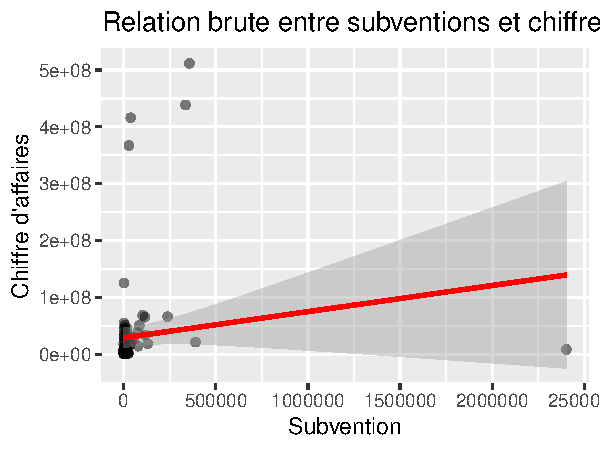
\includegraphics{scdon2-UPV-report-template_sansPython_files/figure-latex/unnamed-chunk-9-1.pdf}

\subsubsection{\texorpdfstring{\textbf{2014}}{2014}}\label{section-2}

\begin{verbatim}
##               Df    Sum Sq   Mean Sq F value Pr(>F)    
## categorie      3 5.252e+19 1.751e+19    1118 <2e-16 ***
## Residuals   2716 4.253e+19 1.566e+16                   
## ---
## Signif. codes:  0 '***' 0.001 '**' 0.01 '*' 0.05 '.' 0.1 ' ' 1
\end{verbatim}

\begin{itemize}
\tightlist
\item
  Détails du test :
\end{itemize}

\medskip

\begin{itemize}
\item
  \textbf{Df (degrés de liberté)} : La variable `categorie' a 3 degrés
  de liberté, ce qui correspond à 4 catégories : Microentreprise, PME,
  ETI, et Grande entreprise. Les résidus ont 2716 degrés de liberté,
  correspondant au nombre de données restantes après l'application des
  catégories.
\item
  \textbf{Sum Sq (somme des carrés)} : Pour la variable `categorie', la
  somme des carrés est de 5.252e+19, ce qui représente la variation
  expliquée par les différences entre les catégories. Pour les résidus,
  la somme des carrés est de 4.253e+19, représentant la variation non
  expliquée par le modèle.
\item
  \textbf{Mean Sq (moyenne des carrés)} : La moyenne des carrés pour
  `categorie' est de 1.751e+19, La moyenne des carrés pour les résidus
  est de 1.566e+16.
\item
  \textbf{F value} : La valeur de F est très élevée, à 1118, ce qui
  montre qu'il existe une grande différence entre les groupes par
  rapport à la variation résiduelle. Une valeur de F élevée signifie que
  les différences entre les groupes sont beaucoup plus grandes que la
  variation interne à chaque groupe.
\item
  \textbf{Pr(\textgreater F)} : La valeur p associée à ce test est
  inférieure à 2e-16, ce qui est bien en dessous du seuil de 0.05. Cela
  montre que les différences entre les catégories sont très
  significatives, ce qui nous permet de rejeter l'hypothèse nulle selon
  laquelle il n'y a pas de différence entre les catégories.
\item
  \textbf{Interprétation des résultats} : Le test ANOVA montre que la
  variable `Chiffres\_d\_affaires\_nets' varie de manière significative
  en fonction de la catégorie d'entreprise (Microentreprise, PME, ETI,
  Grande entreprise). La valeur p très faible (\textless{} 2e-16)
  indique que les moyennes des chiffres d'affaires nets sont
  statistiquement différentes selon les catégories d'entreprises. Cela
  signifie que l'appartenance à une catégorie d'entreprise
  (Microentreprise, PME, ETI, Grande entreprise) a un impact
  significatif sur les chiffres d'affaires nets pour l'année 2014.
\item
  \textbf{Conclusion} : Le test ANOVA confirme que la taille de
  l'entreprise (catégorie) influence le chiffre d'affaires net des
  entreprises en 2014. En comparant les moyennes des différentes
  catégories (Microentreprises, PME, ETI, et Grandes entreprises), on
  peut dire qu'il y a des différences marquées dans les chiffres
  d'affaires entre ces groupes.
\item
  Representation graphique boite a moustaches :
\end{itemize}

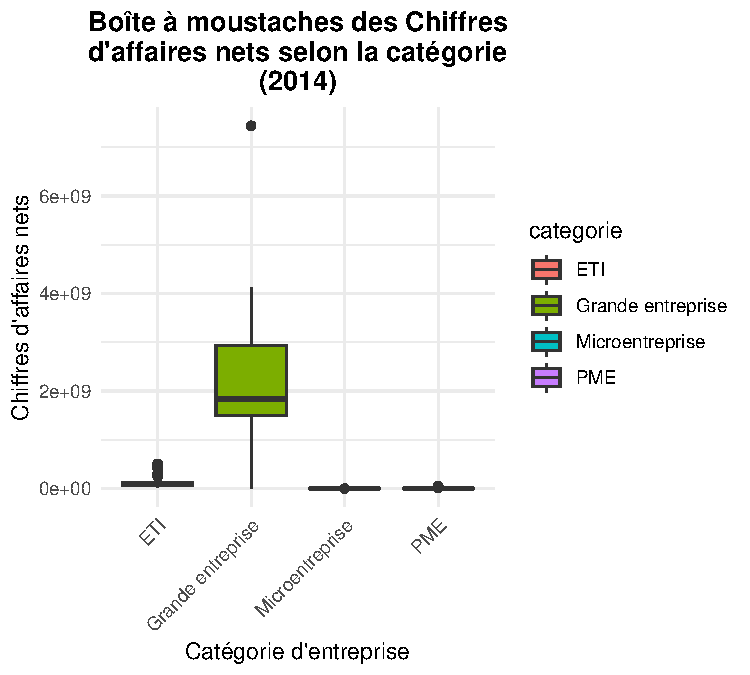
\includegraphics{scdon2-UPV-report-template_sansPython_files/figure-latex/unnamed-chunk-12-1.pdf}
\newpage

\subsubsection{\texorpdfstring{\textbf{2015}}{2015}}\label{section-3}

\begin{verbatim}
##               Df    Sum Sq   Mean Sq F value Pr(>F)    
## categorie      3 2.864e+19 9.546e+18    2780 <2e-16 ***
## Residuals   9588 3.293e+19 3.434e+15                   
## ---
## Signif. codes:  0 '***' 0.001 '**' 0.01 '*' 0.05 '.' 0.1 ' ' 1
\end{verbatim}

\begin{itemize}
\tightlist
\item
  Détails du test :
\end{itemize}

\medskip

\begin{itemize}
\item
  \textbf{Df (Degrés de liberté)} : Le facteur ``categorie'' a 3 degrés
  de liberté, et les résidus (erreurs) ont 9588 degrés de liberté. Cela
  reflète le nombre de groupes comparés (les différentes catégories
  d'entreprises) et la quantité de données disponibles pour les erreurs.
\item
  \textbf{Sum Sq (Somme des carrés)} : La somme des carrés représente la
  variation dans les données. La variation expliquée par la catégorie
  d'entreprise est de 2.864e+19, tandis que la variation résiduelle
  (l'erreur) est de 3.293e+19.
\item
  \textbf{Mean Sq (Moyenne des carrés)} : La moyenne des carrés est
  calculée en divisant la somme des carrés par les degrés de liberté.
  Pour la catégorie, la moyenne des carrés est de 9.546e+18, et pour les
  résidus, elle est de 3.434e+15.
\item
  \textbf{F value} : Le F-value est le rapport entre la variation
  expliquée par les catégories et celle des résidus. Ici, il est de
  2780, ce qui est très élevé, indiquant une différence marquée entre
  les groupes.
\item
  \textbf{Pr(\textgreater F)} : La p-value associée au test F. Elle est
  inférieure à 2e-16, ce qui est très significatif. Cela montre que la
  probabilité que les différences observées soient dues au hasard est
  extrêmement faible.
\item
  \textbf{Test de Signification} : La p-value obtenue est extrêmement
  faible (\textless{} 2e-16), ce qui signifie que l'hypothèse nulle
  (H0), qui stipule qu'il n'y a pas de différence entre les groupes, est
  rejetée. Ainsi, au seuil de 5 \% de signification, nous concluons
  qu'il existe une différence statistiquement significative entre les
  moyennes des chiffres d'affaires nets des différentes catégories
  d'entreprises.
\item
  \textbf{Que signifie cette différence ?} : Les entreprises de
  catégories différentes (comme les Microentreprises, PME, ETI, et
  Grandes entreprises) ont des chiffres d'affaires nets très différents.
  Par exemple, une Microentreprise n'a clairement pas les mêmes
  performances financières qu'une PME ou une Grande entreprise.
\item
  \textbf{Résumé} : En 2015, les chiffres d'affaires nets varient de
  manière significative selon la catégorie d'entreprise. Cela suggère
  que les petites entreprises (comme les Microentreprises) génèrent
  beaucoup moins de chiffre d'affaires net comparées aux entreprises
  plus grandes.
\end{itemize}

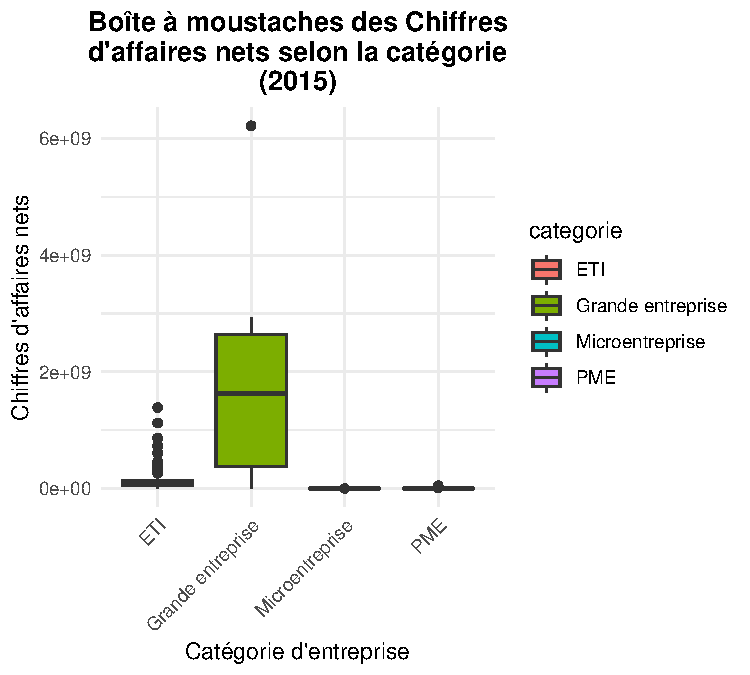
\includegraphics{scdon2-UPV-report-template_sansPython_files/figure-latex/unnamed-chunk-15-1.pdf}

\subsubsection{\texorpdfstring{\textbf{2016}}{2016}}\label{section-4}

\begin{verbatim}
##               Df    Sum Sq   Mean Sq F value Pr(>F)    
## categorie      3 1.092e+19 3.639e+18   200.9 <2e-16 ***
## Residuals   1358 2.460e+19 1.812e+16                   
## ---
## Signif. codes:  0 '***' 0.001 '**' 0.01 '*' 0.05 '.' 0.1 ' ' 1
\end{verbatim}

\medskip

\begin{itemize}
\tightlist
\item
  Détails du test :
\end{itemize}

\medskip

\begin{itemize}
\item
  \textbf{Df (Degrés de liberté)} : Le facteur ``categorie'' a 3 degrés
  de liberté, et les résidus (erreurs) ont 1358 degrés de liberté. Cela
  représente le nombre de groupes comparés (les différentes catégories
  d'entreprises) et la quantité de données restantes pour l'erreur.
\item
  \textbf{Sum Sq (Somme des carrés)} : La somme des carrés représente la
  variation dans les données. La variation expliquée par la catégorie
  d'entreprise est de 1.092e+19, tandis que la variation résiduelle
  (l'erreur) est de 2.460e+19.
\item
  \textbf{Mean Sq (Moyenne des carrés)} : La moyenne des carrés est
  calculée en divisant la somme des carrés par les degrés de liberté.
  Pour la catégorie, la moyenne des carrés est de 3.639e+18, et pour les
  résidus, elle est de 1.812e+16.
\item
  \textbf{F value} : Le F-value est le rapport entre la variation
  expliquée par les catégories et celle des résidus. Ici, il est de
  200.9, ce qui est relativement élevé, indiquant une différence entre
  les groupes.
\item
  \textbf{Pr(\textgreater F)} : La p-value associée au test F. Elle est
  inférieure à 2e-16, ce qui est extrêmement significatif. Cela montre
  que la probabilité que les différences observées soient dues au hasard
  est très faible.
\item
  \textbf{Test de Signification :} La p-value obtenue est extrêmement
  faible (\textless{} 2e-16), ce qui signifie que l'hypothèse nulle
  (H0), qui stipule qu'il n'y a pas de différence entre les groupes, est
  rejetée. Ainsi, au seuil de 5 \% de signification, nous concluons
  qu'il existe une différence statistiquement significative entre les
  moyennes des chiffres d'affaires nets des différentes catégories
  d'entreprises.
\item
  \textbf{Que signifie cette différence ? :} Les entreprises de
  catégories différentes (comme les Microentreprises, PME, ETI, et
  Grandes entreprises) ont des chiffres d'affaires nets très différents.
  Une Microentreprise n'a pas les mêmes performances financières qu'une
  PME ou une Grande entreprise.
\item
  \textbf{Résumé} : En 2016, les chiffres d'affaires nets varient de
  manière significative en fonction de la catégorie d'entreprise. Cela
  suggère que les petites entreprises (comme les Microentreprises)
  génèrent beaucoup moins de chiffre d'affaires net comparées aux
  entreprises plus grandes.
\end{itemize}

\medskip

\begin{itemize}
\tightlist
\item
  Représentation graphique (boîte à moustaches):
\end{itemize}

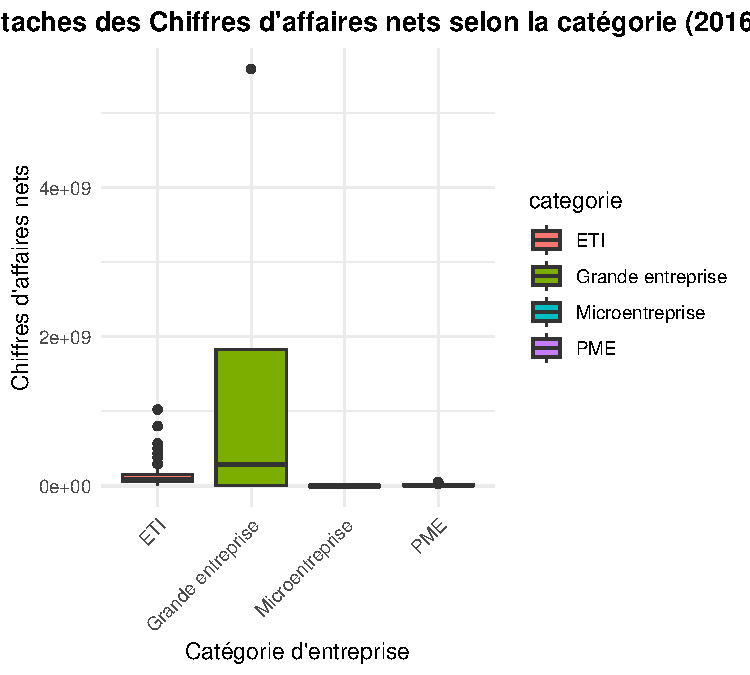
\includegraphics{scdon2-UPV-report-template_sansPython_files/figure-latex/unnamed-chunk-18-1.pdf}

\newpage

\subsection{Conclusion}\label{conclusion}

\medskip

Dans cette analyse, nous avons examiné les différences de chiffre
d'affaires net entre les différentes catégories d'entreprises
\textbf{(Microentreprise, PME, ETI, Grande entreprise)} sur la période
\emph{2012-2016}. Les tests ANOVA ont permis de confirmer que les
différences observées sont statistiquement significatives, ce qui montre
que la taille de l'entreprise a un impact notable sur ses performances
économiques. \medskip Les résultats ont montré que les Microentreprises
génèrent des chiffres d'affaires nettement inférieurs à ceux des PME et
des Grandes entreprises. Les boîtes à moustaches ont illustré
visuellement ces différences, renforçant ainsi les conclusions des tests
statistiques. \medskip En conclusion, cette analyse confirme que la
taille de l'entreprise est un facteur déterminant dans ses résultats
économiques. Ces résultats peuvent être utilisés pour guider des
décisions politiques et stratégiques, notamment pour le soutien aux
entreprises en fonction de leur taille.

\newpage

\section{\texorpdfstring{\textbf{Analyse des subventions et du chiffre
d'affaires}}{Analyse des subventions et du chiffre d'affaires}}\label{analyse-des-subventions-et-du-chiffre-daffaires}

\medskip

L'objectif de cette section est de comprendre si les subventions reçues
par les entreprises françaises ont un impact sur leur chiffre
d'affaires.

Les montants des subventions et du chiffre d'affaires varient énormément
entre les entreprises : certaines ne reçoivent presque rien, d'autres
ont des montants très élevés. Pour rendre les données plus lisibles et
éviter que quelques cas extrêmes ne faussent les résultats, on utilise
une transformation logarithmique. Cela permet d'observer les tendances
de manière plus équilibrée et de voir si, proportionnellement, plus de
subventions entraîne plus de chiffre d'affaires.

\subsubsection{1. Nettoyage et préparation des
données}\label{nettoyage-et-pruxe9paration-des-donnuxe9es}

\medskip

Nous avons utilisé conncetion MySQL pour examiner cette party, voici le
code R:

\medskip

\footnotesize

\begin{Shaded}
\begin{Highlighting}[]
\NormalTok{con }\OtherTok{\textless{}{-}} \FunctionTok{dbConnect}\NormalTok{(}
  \FunctionTok{MySQL}\NormalTok{(),}
  \AttributeTok{user =} \StringTok{"root"}\NormalTok{,}
  \AttributeTok{password =} \StringTok{"root"}\NormalTok{, }\CommentTok{\# même mot de passe créé plus haut}
  \AttributeTok{dbname =} \StringTok{"projet\_L\_2"}\NormalTok{,}
  \AttributeTok{host =} \StringTok{"127.0.0.1"}\NormalTok{,}
  \AttributeTok{port =} \DecValTok{8889}
\NormalTok{)}

\CommentTok{\# Vérifie immédiatement la connexion :}
\CommentTok{\#dbListTables(con)}

\NormalTok{df }\OtherTok{\textless{}{-}} \FunctionTok{dbGetQuery}\NormalTok{(con, }\StringTok{"}
\StringTok{SELECT}
\StringTok{    s.siren,}
\StringTok{    s.denomination,}
\StringTok{    s.town,}
\StringTok{    s.ape,}
\StringTok{    a.ape\_name,}
\StringTok{    cr.year,}
\StringTok{    cr.\textasciigrave{}Chiffres d’affaires nets\textasciigrave{} AS chiffre\_affaires,}
\StringTok{    sb.\textasciigrave{}Subventions d’exploitation\textasciigrave{} AS subvention}
\StringTok{FROM projet\_L\_2.societe s}
\StringTok{JOIN projet\_L\_2.apegen a}
\StringTok{  ON s.ape = a.ape}
\StringTok{JOIN projet\_L\_2.compte\_resultat cr}
\StringTok{  ON s.siren = cr.siren}
\StringTok{JOIN projet\_L\_2.subvention sb}
\StringTok{  ON s.siren = sb.siren AND cr.year = sb.year}
\StringTok{WHERE cr.\textasciigrave{}Chiffres d’affaires nets\textasciigrave{} IS NOT NULL}
\StringTok{  AND sb.\textasciigrave{}Subventions d’exploitation\textasciigrave{} IS NOT NULL}
\StringTok{"}\NormalTok{)}
\end{Highlighting}
\end{Shaded}

\normalsize

\newpage

\begin{Shaded}
\begin{Highlighting}[]
\FunctionTok{library}\NormalTok{(dplyr)}
\FunctionTok{library}\NormalTok{(ggplot2)}

\CommentTok{\# Nettoyage}
\NormalTok{df\_clean }\OtherTok{\textless{}{-}}\NormalTok{ df }\SpecialCharTok{\%\textgreater{}\%}
  \FunctionTok{mutate}\NormalTok{(}
    \AttributeTok{chiffre\_affaires =} \FunctionTok{as.numeric}\NormalTok{(}\FunctionTok{gsub}\NormalTok{(}\StringTok{"[\^{}0{-}9]"}\NormalTok{, }\StringTok{""}\NormalTok{, chiffre\_affaires)),}
    \AttributeTok{subvention =} \FunctionTok{as.numeric}\NormalTok{(}\FunctionTok{gsub}\NormalTok{(}\StringTok{"[\^{}0{-}9]"}\NormalTok{, }\StringTok{""}\NormalTok{, subvention))}
\NormalTok{  ) }\SpecialCharTok{\%\textgreater{}\%}
  \FunctionTok{filter}\NormalTok{(}\SpecialCharTok{!}\FunctionTok{is.na}\NormalTok{(chiffre\_affaires) }\SpecialCharTok{\&} \SpecialCharTok{!}\FunctionTok{is.na}\NormalTok{(subvention))}

\CommentTok{\# Création des colonnes logarithmiques}
\NormalTok{df\_log }\OtherTok{\textless{}{-}}\NormalTok{ df\_clean }\SpecialCharTok{\%\textgreater{}\%}
  \FunctionTok{filter}\NormalTok{(chiffre\_affaires }\SpecialCharTok{\textgreater{}} \DecValTok{0}\NormalTok{, subvention }\SpecialCharTok{\textgreater{}} \DecValTok{0}\NormalTok{) }\SpecialCharTok{\%\textgreater{}\%}
  \FunctionTok{mutate}\NormalTok{(}
    \AttributeTok{log\_CA =} \FunctionTok{log10}\NormalTok{(chiffre\_affaires),}
    \AttributeTok{log\_subvention =} \FunctionTok{log10}\NormalTok{(subvention)}
\NormalTok{  )}

\CommentTok{\# Régression log{-}log}
\NormalTok{modele\_log }\OtherTok{\textless{}{-}} \FunctionTok{lm}\NormalTok{(log\_CA }\SpecialCharTok{\textasciitilde{}}\NormalTok{ log\_subvention, }\AttributeTok{data =}\NormalTok{ df\_log)}
\FunctionTok{summary}\NormalTok{(modele\_log)}
\end{Highlighting}
\end{Shaded}

\begin{verbatim}
## 
## Call:
## lm(formula = log_CA ~ log_subvention, data = df_log)
## 
## Residuals:
##      Min       1Q   Median       3Q      Max 
## -1.35059 -0.46289  0.02854  0.46093  1.64308 
## 
## Coefficients:
##                Estimate Std. Error t value Pr(>|t|)    
## (Intercept)     5.11391    0.31714  16.125  < 2e-16 ***
## log_subvention  0.44712    0.08262   5.412 4.59e-07 ***
## ---
## Signif. codes:  0 '***' 0.001 '**' 0.01 '*' 0.05 '.' 0.1 ' ' 1
## 
## Residual standard error: 0.6789 on 96 degrees of freedom
## Multiple R-squared:  0.2337, Adjusted R-squared:  0.2258 
## F-statistic: 29.28 on 1 and 96 DF,  p-value: 4.589e-07
\end{verbatim}

\normalsize

\newpage

\subsubsection{2. Analyse univariée}\label{analyse-univariuxe9e}

\medskip

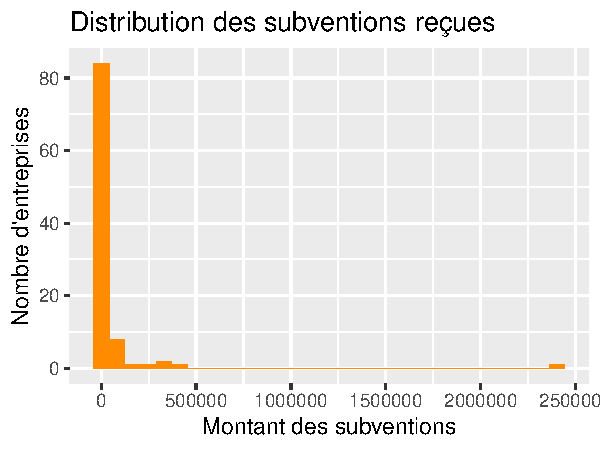
\includegraphics{scdon2-UPV-report-template_sansPython_files/figure-latex/unnamed-chunk-21-1.pdf}

\begin{quote}
La majorité des entreprises reçoivent de petites subventions.
Quelques-unes, plus rares, touchent des montants bien plus élevés.
\end{quote}

\medskip

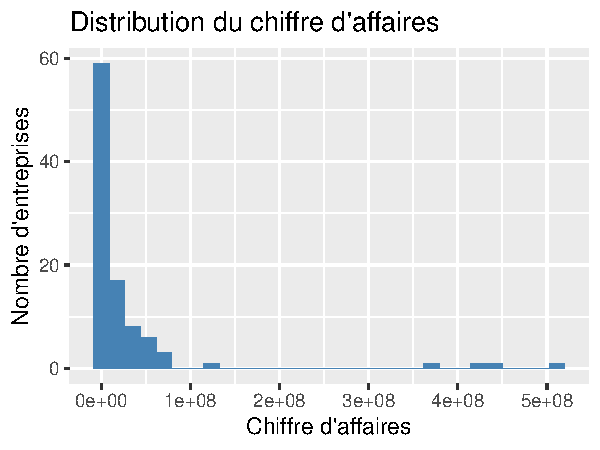
\includegraphics{scdon2-UPV-report-template_sansPython_files/figure-latex/unnamed-chunk-22-1.pdf}

\begin{quote}
Le chiffre d'affaires est aussi très variable, certaines entreprises
réalisant plusieurs dizaines de millions d'euros.
\end{quote}

\medskip

\subsubsection{3. Analyse bivariée
brute}\label{analyse-bivariuxe9e-brute}

\medskip

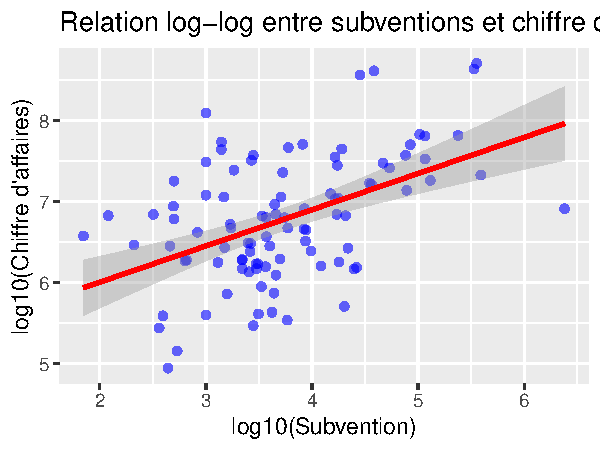
\includegraphics{scdon2-UPV-report-template_sansPython_files/figure-latex/unnamed-chunk-23-1.pdf}

\begin{quote}
À première vue, il n'y a pas de lien clair entre les subventions et le
chiffre d'affaires. Le graphique montre beaucoup de dispersion, ce qui
empêche une vraie lecture de tendance.
\end{quote}

\medskip

\subsubsection{4. Régression log-log :
Visualisation}\label{ruxe9gression-log-log-visualisation}

\medskip

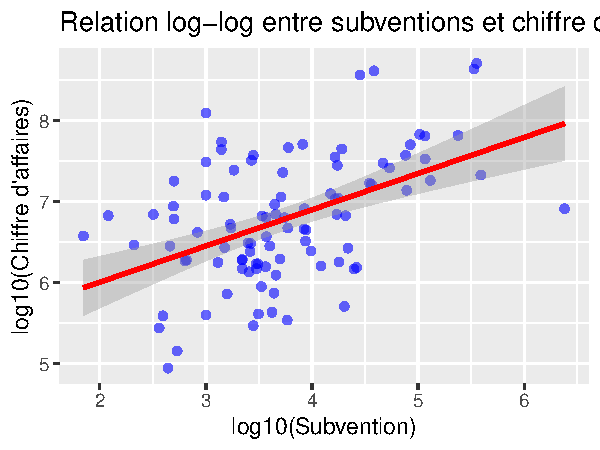
\includegraphics{scdon2-UPV-report-template_sansPython_files/figure-latex/unnamed-chunk-24-1.pdf}

\begin{quote}
Une fois les données transformées en logarithme, une tendance apparaît :
les entreprises qui reçoivent plus de subventions ont, en moyenne, un
chiffre d'affaires plus élevé. La relation est significative et le
modèle indique qu'une augmentation de 10\% des subventions correspond à
une hausse d'environ 4,5\% du chiffre d'affaires.
\end{quote}

\medskip

\subsubsection{Conclusion}\label{conclusion-1}

\medskip

En conclusion, même si à l'échelle brute le lien entre subventions et
chiffre d'affaires n'est pas visible, la transformation log-log montre
qu'il existe une \textbf{relation proportionnelle significative}. Cela
signifie que les subventions peuvent avoir un impact positif mesurable
sur le développement économique des entreprises, en particulier si l'on
considère les effets relatifs plutôt que les montants absolus. sans
refinancement : Total des charges financières = 0

\newpage

\section{\texorpdfstring{\textbf{Analyser des entreprises en fonction de
leur localisation
géographique}}{Analyser des entreprises en fonction de leur localisation géographique}}\label{analyser-des-entreprises-en-fonction-de-leur-localisation-guxe9ographique}

\bigskip

L'objectif de cette étude est d'analyser des entreprises en France à
partir de données financières entre 2012 et 2016. Nous avons examiné
\textbf{le chiffre d'affaires net}, \textbf{le résultat d'exploitation}.
Des entreprises et a été examinée par \textbf{année} et par
\textbf{region}. La base de données ne contenait que des codes postaux.
Nous avons d'abord regroupé les départements puis les régions en
fonction des deux chiffres du code postal.Nous avons examiné chaque
année indépendamment.

\medskip

Dans ce chapite pour analyse univarie, nous allons presenter l'annes
2015 car l'année avec le plus de données est 2015. Nous avons constaté
que les différences et les incohérences dans la taille des données selon
les années et les régions constituaient un obstacle.

\medskip

\begin{figure}
\centering
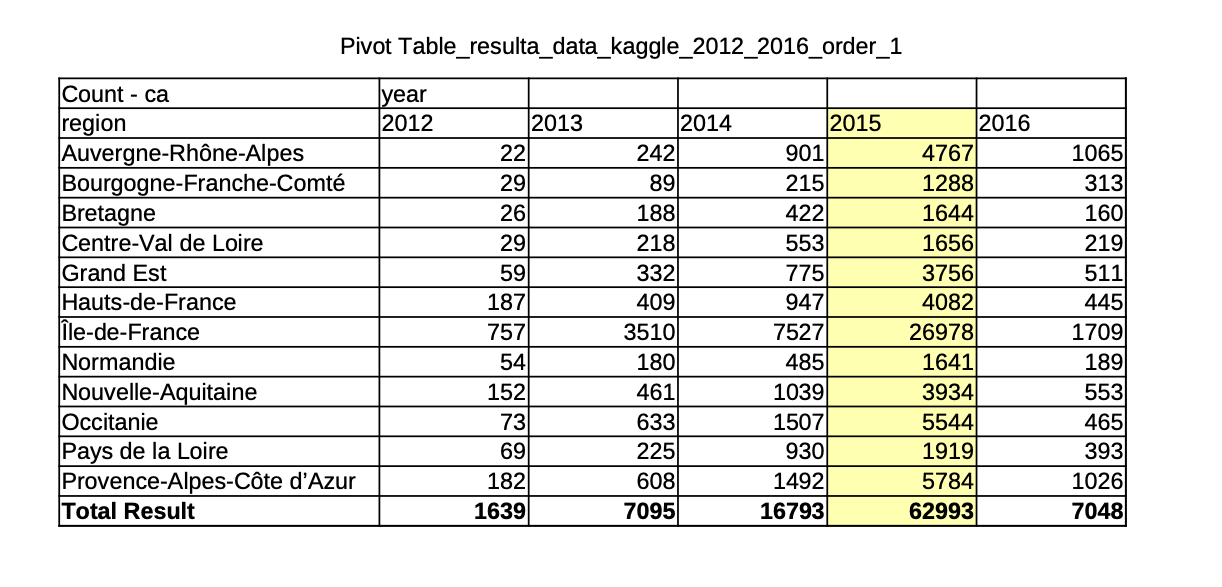
\includegraphics[width=10cm,height=5cm]{image_sql/image_independant/count_region-ca.png}
\caption{Pivot Table}\label{Pivot}
\end{figure}

\medskip

\subsection{Préparation des
données}\label{pruxe9paration-des-donnuxe9es}

\medskip

\begin{enumerate}
\def\labelenumi{\arabic{enumi})}
\tightlist
\item
  Un fichier CSV (créé par code R) contenant les données financières de
  l'entreprise de 2012 à 2016 a été utilisé
\end{enumerate}

\small

\normalsize

\begin{enumerate}
\def\labelenumi{\arabic{enumi})}
\setcounter{enumi}{1}
\tightlist
\item
  Les Variables sont utilise:
\end{enumerate}

\begin{longtable}[]{@{}ll@{}}
\toprule\noalign{}
Variable & source \\
\midrule\noalign{}
\endhead
\bottomrule\noalign{}
\endlastfoot
Year & Datakagle.csv \\
Siren & Datakagle.csv \\
résultat d'exploitation & Datakagle.csv \\
chiffres d'affaires nets & Datakagle.csv \\
code\_postal & Datakagle.csv \\
rentabilite & créé \\
categorie\_rentabilite & créé \\
Department & créé \\
region & créé \\
\end{longtable}

\medskip

\begin{enumerate}
\def\labelenumi{\arabic{enumi})}
\setcounter{enumi}{2}
\tightlist
\item
  Création d'une variable catégorielle : La valeur de rentabilité est
  divisée dans les classes suivantes :
\end{enumerate}

\[
      \text{rentabilité} = \frac{\text{résultat d'exploitation}}{\text{chiffres d’affaires nets}}
\]

\medskip

\begin{longtable}[]{@{}ll@{}}
\caption{Classification des entreprises selon leur
rentabilité}\tabularnewline
\toprule\noalign{}
Intervalle de rentabilité & Catégorie \\
\midrule\noalign{}
\endfirsthead
\toprule\noalign{}
Intervalle de rentabilité & Catégorie \\
\midrule\noalign{}
\endhead
\bottomrule\noalign{}
\endlastfoot
Rentabilité \(< 0\) & En perte \\
\(0 \leq\) Rentabilité \(< 0{,}1\) & Faible rentabilité \\
\(0{,}1 \leq\) Rentabilité \(< 0{,}3\) & Rentabilité moyenne \\
Rentabilité \(\geq 0{,}3\) & Haute rentabilité \\
\end{longtable}

\medskip

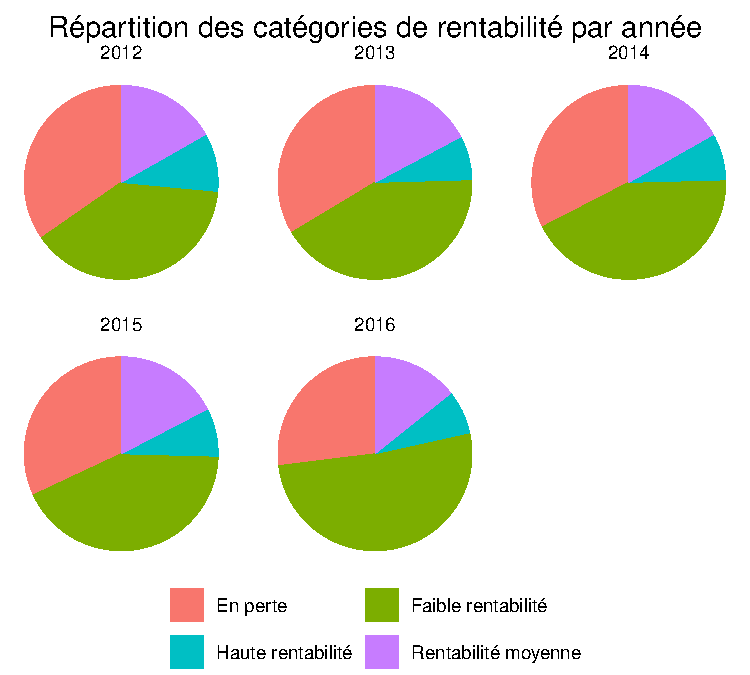
\includegraphics{scdon2-UPV-report-template_sansPython_files/figure-latex/rentabilite-1.pdf}

\newpage

\subsection{Analyse Univarie}\label{analyse-univarie}

\medskip

\subsubsection{Chifre d'afffaire}\label{chifre-dafffaire}

\begin{longtable}[t]{lrrrrr}
\caption{\label{tab:chiffre_affaire_summary_2015}Résumé des statistiques du chiffre d'affaires nets (en millions d'euros) – 2015}\\
\toprule
region & avarage & median & min & max & ecart\_type\\
\midrule
\endfirsthead
\caption[]{Résumé des statistiques du chiffre d'affaires nets (en millions d'euros) – 2015 \textit{(continued)}}\\
\toprule
region & avarage & median & min & max & ecart\_type\\
\midrule
\endhead

\endfoot
\bottomrule
\endlastfoot
Auvergne-Rhône-Alpes & 3.18 & 0.33 & -0.06 & 1083.39 & 25.26\\
Bourgogne-Franche-Comté & 4.21 & 0.56 & 0.00 & 436.49 & 20.71\\
Bretagne & 11.57 & 0.74 & 0.00 & 2938.86 & 101.94\\
Centre-Val de Loire & 4.06 & 0.44 & -0.12 & 531.87 & 23.78\\
Grand Est & 4.36 & 0.53 & -0.04 & 1584.02 & 36.31\\
\addlinespace
Hauts-de-France & 3.26 & 0.49 & -0.11 & 537.71 & 17.26\\
Normandie & 4.52 & 0.59 & -0.01 & 1155.42 & 34.62\\
Nouvelle-Aquitaine & 3.51 & 0.44 & -0.05 & 1788.57 & 35.47\\
Occitanie & 2.17 & 0.36 & -0.14 & 360.82 & 10.56\\
Pays de la Loire & 10.93 & 0.78 & -0.01 & 2729.00 & 90.24\\
\addlinespace
Provence-Alpes-Côte d'Azur & 1.46 & 0.35 & -6.59 & 366.13 & 7.17\\
Île-de-France & 3.91 & 0.35 & -0.31 & 6217.25 & 64.37\\*
\end{longtable}

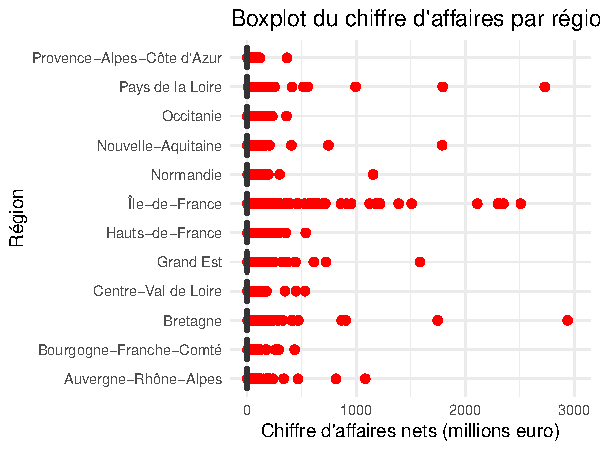
\includegraphics{scdon2-UPV-report-template_sansPython_files/figure-latex/chiffre_affaire_graph_2015-1.pdf}

\newpage

\subsubsection{Resultat d'Explation}\label{resultat-dexplation}

\begin{longtable}[t]{lrrrrr}
\caption{\label{tab:resultat_exp_summary_2015}Résumé des statistiques du Résultat d'exploitation (en millions d'euros) – 2015}\\
\toprule
region & avarage & median & min & max & ecart\_type\\
\midrule
\endfirsthead
\caption[]{Résumé des statistiques du Résultat d'exploitation (en millions d'euros) – 2015 \textit{(continued)}}\\
\toprule
region & avarage & median & min & max & ecart\_type\\
\midrule
\endhead

\endfoot
\bottomrule
\endlastfoot
Auvergne-Rhône-Alpes & 3.18 & 0.33 & -0.06 & 1083.39 & 25.26\\
Bourgogne-Franche-Comté & 4.21 & 0.56 & 0.00 & 436.49 & 20.71\\
Bretagne & 11.57 & 0.74 & 0.00 & 2938.86 & 101.94\\
Centre-Val de Loire & 4.06 & 0.44 & -0.12 & 531.87 & 23.78\\
Grand Est & 4.36 & 0.53 & -0.04 & 1584.02 & 36.31\\
\addlinespace
Hauts-de-France & 3.26 & 0.49 & -0.11 & 537.71 & 17.26\\
Normandie & 4.52 & 0.59 & -0.01 & 1155.42 & 34.62\\
Nouvelle-Aquitaine & 3.51 & 0.44 & -0.05 & 1788.57 & 35.47\\
Occitanie & 2.17 & 0.36 & -0.14 & 360.82 & 10.56\\
Pays de la Loire & 10.93 & 0.78 & -0.01 & 2729.00 & 90.24\\
\addlinespace
Provence-Alpes-Côte d'Azur & 1.46 & 0.35 & -6.59 & 366.13 & 7.17\\
Île-de-France & 3.91 & 0.35 & -0.31 & 6217.25 & 64.37\\*
\end{longtable}

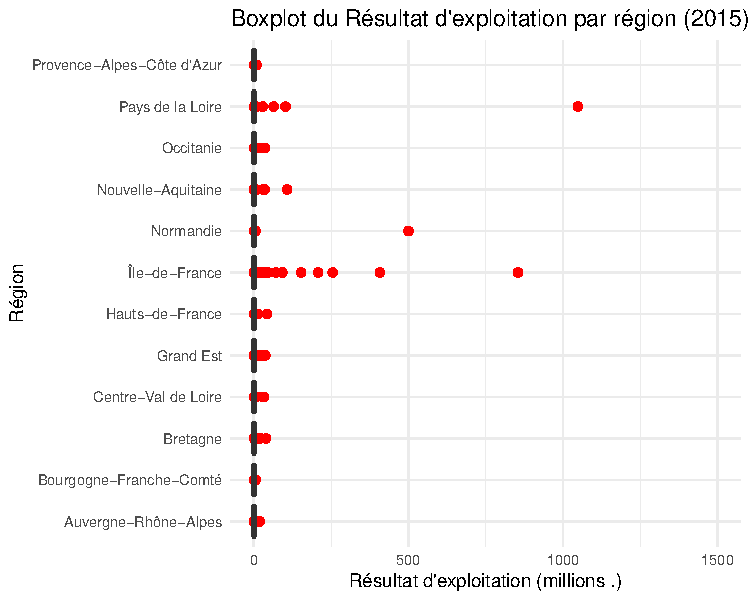
\includegraphics{scdon2-UPV-report-template_sansPython_files/figure-latex/resulta_graph_2015-1.pdf}

\newpage

\subsection{Analyse Bivarie}\label{analyse-bivarie}

\medskip

\subsubsection{Chiffre d'affaires nets et Résultat
d'exploitation}\label{chiffre-daffaires-nets-et-ruxe9sultat-dexploitation}

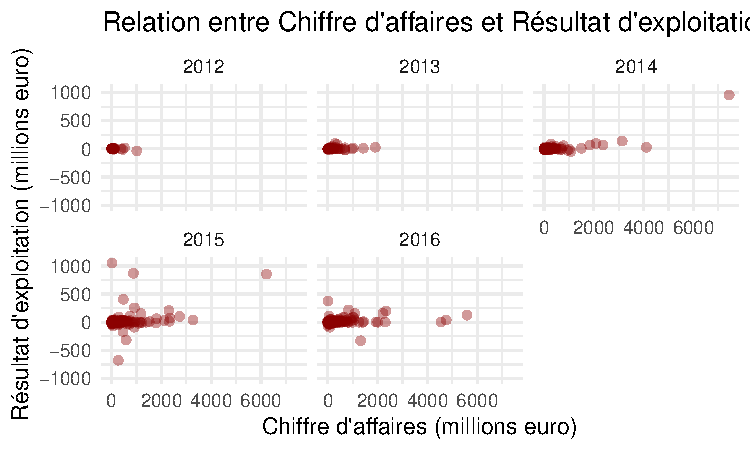
\includegraphics{scdon2-UPV-report-template_sansPython_files/figure-latex/nuage_point_anness-1.pdf}

\subsubsection{Coefficient de corrélation de
Pearson}\label{coefficient-de-corruxe9lation-de-pearson}

\medskip

\begin{longtable}[]{@{}lll@{}}
\toprule\noalign{}
Année & Corrélation (Pearson) & Interprétation \\
\midrule\noalign{}
\endhead
\bottomrule\noalign{}
\endlastfoot
2012 & -0.45 & Corrélation négative modérée \\
2013 & 0.35 & Relation positive modérée \\
2014 & 0.80 & Forte corrélation positive \\
2015 & 0.38 & Tendance positive similaire à 2013 \\
2016 & 0.29 & Corrélation positive mais faible \\
\end{longtable}

\medskip

La corrélation doit être comprise entre \textbf{-1 et 1}, donc les
valeurs que nous avons trouvées sont correctes. On peut dire qu'en 2012,
il existe une relation \textbf{négative} entre les deux variables. Pour
les années 2013, 2015 et 2016, la corrélation est \textbf{faible mais
positive} : cela signifie que lorsque le chiffre d'affaires augmente, le
résultat d'exploitation a tendance à augmenter également. En 2014, on
observe une \textbf{forte} corrélation positive, ce qui indique une
relation claire entre les deux variables : elles ont tendance à évoluer
dans le même sens, c'est-à-dire à augmenter en même temps.

\newpage

\subsubsection{Regreation droit}\label{regreation-droit}

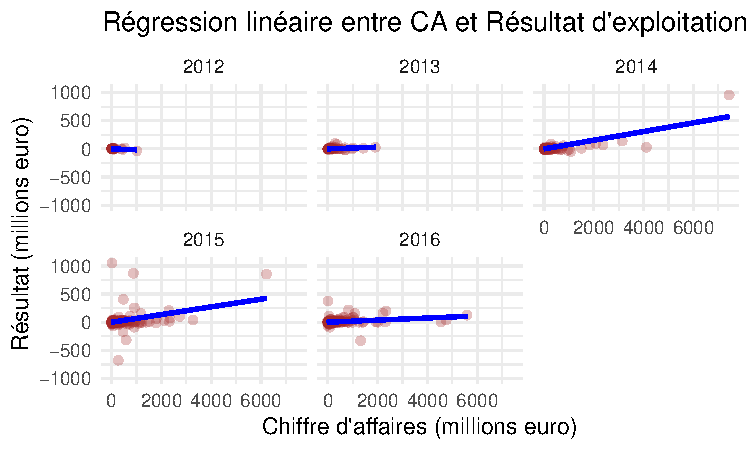
\includegraphics{scdon2-UPV-report-template_sansPython_files/figure-latex/reg_droit-1.pdf}

\medskip

\textbf{Formuler les hypothèses :}

\bigskip

\begin{itemize}
\tightlist
\item
  Hypothèse nulle (H\textsubscript{0}) : La répartition du chiffre
  d'affaires net et du résultat d'exploitation ne varie pas selon les
  régions. \medskip
\item
  Hypothèse alternative (H\textsubscript{1}) : Il existe une différence
  significative du chiffre d'affaires net et du résultat d'exploitation
  entre les régions.
\end{itemize}

\begin{verbatim}
##      Annee F_value     p_value   Decision
## 2012  2012   11.49 0.000000000 H0 rejetée
## 2013  2013    6.25 0.000000000 H0 rejetée
## 2014  2014    3.77 0.000020167 H0 rejetée
## 2015  2015    7.46 0.000000000 H0 rejetée
## 2016  2016    2.76 0.001434238 H0 rejetée
\end{verbatim}

\bigskip

\begin{verbatim}
##      Annee F_value p_value       Decision
## 2012  2012    0.72  0.7195 H0 non rejetée
## 2013  2013    0.61  0.8213 H0 non rejetée
## 2014  2014    0.18  0.9987 H0 non rejetée
## 2015  2015    1.95  0.0289     H0 rejetée
## 2016  2016    0.44  0.9379 H0 non rejetée
\end{verbatim}

\subsubsection{Conclusion}\label{conclusion-2}

\newpage

\section{\texorpdfstring{\textbf{La variation de la rentabilité selon le
secteur d'activité des
entreprises}}{La variation de la rentabilité selon le secteur d'activité des entreprises}}\label{la-variation-de-la-rentabilituxe9-selon-le-secteur-dactivituxe9-des-entreprises}

\bigskip

\textbf{Variables} : le code APE (le secteur d'activité des entreprises)
+ Chiffres d'affaires nets

\subsection{Étapes pour créer une visualisation
:}\label{uxe9tapes-pour-cruxe9er-une-visualisation}

\subsubsection{Catégorisation des entreprises par secteur d'activité
:}\label{catuxe9gorisation-des-entreprises-par-secteur-dactivituxe9}

\subsubsection{Visualisation :}\label{visualisation}

\textbf{Boxplot} : Visualiser la distribution des chiffres d'affaires
nets pour chaque secteur d'activité.\textbackslash{} \textbf{Diagramme
en barres} : Montrer la moyenne des chiffres d'affaires nets par secteur
d'activité.

\subsubsection{Test Statistique (ANOVA)
:}\label{test-statistique-anova-1}

\textbf{Chauque un/e doit proposer son text :) }

Dans cette partie, vous pourrez utiliser les outils et méthodes vus au
semestre précédent pour analyser les liens entre les variables.

Pour cela, vous pourrez utiliser les tests du \(\chi^2\), test du
coefficient de corrélation linéaire, test d'Anova, la droite de
régression linéaire.

Vous pourrez également proposer des modèles pour faire du clustering
(k-means, CAH), de la classification (K plus proches voisins par
exemple) comme vu en Science des données 1.

\newpage

\chapter{Discussion}\label{discussion}

Placer les résultats que vous avez obtenus dans le chapitre précédent en
perspective par rapport au problème étudié.

\chapter{Conclusion et perspectives}\label{conclusion-et-perspectives}

Quelles sont les conclusions principales? Quelles sont vos
recommandations pour le commanditaire? Quelles analyses subséquentes
pourraient être faites dans le futur?

\bigskip

On attend de vous deux types de perspectives : des perspectives à court
terme pour améliorer rapidement votre approche et des perspectives à
plus long terme qu'elles soient liées à la science des données ou au
domaine métier pour lequel vous avez travaillé.

\bigskip

Lister également les difficultés rencontrées dans la partie BD (e.g.,
taille de la base, manque de données, \ldots) et dans la partie
statistique.

\chapter*{Bibliographie}\label{bibliographie}
\addcontentsline{toc}{chapter}{Bibliographie}

\phantomsection\label{refs}
\begin{CSLReferences}{0}{1}
\end{CSLReferences}

\bibliographystyle{elsarticle-harv}
\bibliography{references}

\chapter*{Annexes}\label{annexes}
\addcontentsline{toc}{chapter}{Annexes}

Il faut utiliser les annexes de façon judicieuse. C'est ici que l'on
place des résultats trop volumineux pour apparaître dans le corps du
rapport. Ou bien des résultats (e.g., graphiques) moins intéressants que
les autres. Cela permet de limiter le nombre de pages du coeur du
rapport, et d'ajouter des détails dans cette partie pour le lecteur
désireux d'en savoir plus.

\section*{\texorpdfstring{\textbf{Codes}}{Codes}}\label{codes}
\addcontentsline{toc}{section}{\textbf{Codes}}

\tiny

\begin{Shaded}
\begin{Highlighting}[]
\CommentTok{\#Charger la bibliothèque}
\FunctionTok{library}\NormalTok{(readr)}

\CommentTok{\#Lire le fichier CSV}
\NormalTok{data\_kaggle }\OtherTok{\textless{}{-}} \FunctionTok{read\_csv}\NormalTok{(}\StringTok{"csv/data\_kaggle.csv"}\NormalTok{)}

\CommentTok{\#Fonction pour calculer la rentabilité (PAS de référence directe à data\_kaggle dans les paramètres)}
\NormalTok{fonction\_rentabilite }\OtherTok{\textless{}{-}} \ControlFlowTok{function}\NormalTok{(resultat\_financier, ca\_net) \{}
  \ControlFlowTok{if}\NormalTok{ (}\SpecialCharTok{!}\FunctionTok{is.na}\NormalTok{(resultat\_financier) }\SpecialCharTok{\&\&} \SpecialCharTok{!}\FunctionTok{is.na}\NormalTok{(ca\_net) }\SpecialCharTok{\&\&}\NormalTok{ ca\_net }\SpecialCharTok{!=} \DecValTok{0}\NormalTok{) \{}
    \FunctionTok{return}\NormalTok{(resultat\_financier }\SpecialCharTok{/}\NormalTok{ ca\_net)}
\NormalTok{  \} }\ControlFlowTok{else}\NormalTok{ \{}
    \FunctionTok{return}\NormalTok{(}\ConstantTok{NA}\NormalTok{)}
\NormalTok{  \}}
\NormalTok{\}}

\CommentTok{\#Appliquer la fonction ligne par ligne}
\NormalTok{data\_kaggle}\SpecialCharTok{$}\NormalTok{rentabilite }\OtherTok{\textless{}{-}} \FunctionTok{apply}\NormalTok{(data\_kaggle, }\DecValTok{1}\NormalTok{, }\ControlFlowTok{function}\NormalTok{(row) \{}
\NormalTok{  resultat }\OtherTok{\textless{}{-}} \FunctionTok{as.numeric}\NormalTok{(row[}\StringTok{"Résultat financier"}\NormalTok{])}
\NormalTok{  ca }\OtherTok{\textless{}{-}} \FunctionTok{as.numeric}\NormalTok{(row[}\StringTok{"Chiffres d’affaires nets"}\NormalTok{])}
  \FunctionTok{return}\NormalTok{(}\FunctionTok{fonction\_rentabilite}\NormalTok{(resultat, ca))}
\NormalTok{\})}

\CommentTok{\#Sauvegarder le résultat dans un nouveau fichier CSV}
\FunctionTok{write.csv}\NormalTok{(data\_kaggle, }
          \StringTok{"csv/data\_kaggle\_new.csv"}\NormalTok{, }
          \AttributeTok{row.names =} \ConstantTok{FALSE}\NormalTok{)}

\CommentTok{\#Affichage pour vérification}
\FunctionTok{View}\NormalTok{(data\_kaggle)}
\NormalTok{data\_kaggle}\SpecialCharTok{$}\FunctionTok{rentabilite}\NormalTok{()}
\NormalTok{annee\_2012}\OtherTok{\textless{}{-}}\NormalTok{data\_kaggle}\SpecialCharTok{$}\NormalTok{year[]}
\NormalTok{annee\_2012}


\FunctionTok{install.packages}\NormalTok{(}\StringTok{"sqldf"}\NormalTok{)}
\FunctionTok{library}\NormalTok{(sqldf)}

\NormalTok{result }\OtherTok{\textless{}{-}} \FunctionTok{sqldf}\NormalTok{(}\StringTok{"SELECT * FROM data\_kaggle WHERE year = 2012"}\NormalTok{)}
\NormalTok{result}
\FunctionTok{head}\NormalTok{(result)}
\NormalTok{annee\_2012}\OtherTok{\textless{}{-}}\FunctionTok{sqldf}\NormalTok{(}\StringTok{"SELECT* from data\_kaggle WHERE year=2012"}\NormalTok{)}
\FunctionTok{View}\NormalTok{(annee\_2012)}
\NormalTok{annee\_2013}\OtherTok{\textless{}{-}}\FunctionTok{sqldf}\NormalTok{(}\StringTok{"SELECT* from data\_kaggle WHERE year=2013"}\NormalTok{)}
\NormalTok{annee\_2014}\OtherTok{\textless{}{-}}\FunctionTok{sqldf}\NormalTok{(}\StringTok{"SELECT* from data\_kaggle WHERE year=2014"}\NormalTok{)}
\NormalTok{annee\_2015}\OtherTok{\textless{}{-}}\FunctionTok{sqldf}\NormalTok{(}\StringTok{"SELECT* from data\_kaggle WHERE year=2015"}\NormalTok{)}
\NormalTok{annee\_2016}\OtherTok{\textless{}{-}}\FunctionTok{sqldf}\NormalTok{(}\StringTok{"SELECT* from data\_kaggle WHERE year=2016"}\NormalTok{)}
\FunctionTok{cor}\NormalTok{(annee\_2012}\SpecialCharTok{$}\NormalTok{rentabilite,annee\_2012}\SpecialCharTok{$}\StringTok{\textasciigrave{}}\AttributeTok{Impôts, taxes et versements assimilés}\StringTok{\textasciigrave{}}\NormalTok{,}\AttributeTok{use =} \StringTok{"complete.obs"}\NormalTok{)}
\FunctionTok{plot}\NormalTok{(annee\_2012}\SpecialCharTok{$}\NormalTok{rentabilite,annee\_2012}\SpecialCharTok{$}\StringTok{\textasciigrave{}}\AttributeTok{Impôts, taxes et versements assimilés}\StringTok{\textasciigrave{}}\NormalTok{)}
\CommentTok{\# Table 1 : Société}
\CommentTok{\# Combinaison des 100 premières lignes de chaque sous{-}ensemble}
\NormalTok{sous\_ensemble }\OtherTok{\textless{}{-}} \FunctionTok{rbind}\NormalTok{(}
\NormalTok{  annee\_2012[}\DecValTok{1}\SpecialCharTok{:}\DecValTok{100}\NormalTok{, ],}
\NormalTok{  annee\_2013[}\DecValTok{1}\SpecialCharTok{:}\DecValTok{100}\NormalTok{, ],}
\NormalTok{  annee\_2014[}\DecValTok{1}\SpecialCharTok{:}\DecValTok{100}\NormalTok{, ],}
\NormalTok{  annee\_2015[}\DecValTok{1}\SpecialCharTok{:}\DecValTok{100}\NormalTok{, ],}
\NormalTok{  annee\_2016[}\DecValTok{1}\SpecialCharTok{:}\DecValTok{100}\NormalTok{, ]}
\NormalTok{)}
\FunctionTok{View}\NormalTok{(sous\_ensemble)}

\CommentTok{\# Sélection des colonnes souhaitées}
\NormalTok{societe }\OtherTok{\textless{}{-}}\NormalTok{ sous\_ensemble[, }\FunctionTok{c}\NormalTok{(}\StringTok{"siren"}\NormalTok{, }\StringTok{"denomination"}\NormalTok{, }\StringTok{"postal\_code"}\NormalTok{, }\StringTok{"town"}\NormalTok{, }\StringTok{"ape"}\NormalTok{)]}
\FunctionTok{View}\NormalTok{(societe)}
\FunctionTok{write\_csv}\NormalTok{(societe, }\StringTok{"csv/societe.csv"}\NormalTok{)}

\CommentTok{\# Table 2 : Subventions}
\NormalTok{sous\_ensemble\_2 }\OtherTok{\textless{}{-}} \FunctionTok{rbind}\NormalTok{(}
\NormalTok{  annee\_2012[}\DecValTok{1}\SpecialCharTok{:}\DecValTok{100}\NormalTok{, ],}
\NormalTok{  annee\_2013[}\DecValTok{1}\SpecialCharTok{:}\DecValTok{100}\NormalTok{, ],}
\NormalTok{  annee\_2014[}\DecValTok{1}\SpecialCharTok{:}\DecValTok{100}\NormalTok{, ],}
\NormalTok{  annee\_2015[}\DecValTok{1}\SpecialCharTok{:}\DecValTok{100}\NormalTok{, ],}
\NormalTok{  annee\_2016[}\DecValTok{1}\SpecialCharTok{:}\DecValTok{100}\NormalTok{, ]}
\NormalTok{)}
\NormalTok{subventions}\OtherTok{\textless{}{-}}\NormalTok{sous\_ensemble\_2[, }\FunctionTok{c}\NormalTok{(}\StringTok{"year"}\NormalTok{,}\StringTok{"siren"}\NormalTok{, }\StringTok{"Subventions d’exploitation"}\NormalTok{)]}


\FunctionTok{write\_csv}\NormalTok{(subventions, }\StringTok{"csv/subvention.csv"}\NormalTok{)}

\CommentTok{\# Table 3 : ApeGen}
\NormalTok{sous\_ensemble\_3 }\OtherTok{\textless{}{-}} \FunctionTok{rbind}\NormalTok{(}
\NormalTok{  annee\_2012[}\DecValTok{1}\SpecialCharTok{:}\DecValTok{100}\NormalTok{, ],}
\NormalTok{  annee\_2013[}\DecValTok{1}\SpecialCharTok{:}\DecValTok{100}\NormalTok{, ],}
\NormalTok{  annee\_2014[}\DecValTok{1}\SpecialCharTok{:}\DecValTok{100}\NormalTok{, ],}
\NormalTok{  annee\_2015[}\DecValTok{1}\SpecialCharTok{:}\DecValTok{100}\NormalTok{, ],}
\NormalTok{  annee\_2016[}\DecValTok{1}\SpecialCharTok{:}\DecValTok{100}\NormalTok{, ]}
\NormalTok{)}


\NormalTok{apegen}\OtherTok{\textless{}{-}}\NormalTok{sous\_ensemble\_3[, }\FunctionTok{c}\NormalTok{(}\StringTok{"ape"}\NormalTok{, }\StringTok{"ape\_name"}\NormalTok{, }\StringTok{"ape\_len"}\NormalTok{, }\StringTok{"ape\_division"}\NormalTok{, }\StringTok{"ape\_groupe"}\NormalTok{, }\StringTok{"ape\_classe"}\NormalTok{, }\StringTok{"ape\_sous\_classe"}\NormalTok{)]}
\FunctionTok{write\_csv}\NormalTok{(apegen, }\StringTok{"csv/apegen.csv"}\NormalTok{)}

\CommentTok{\# Table 4 : Chiffre d\textquotesingle{}Affaires}
\NormalTok{sous\_ensemble\_4}\OtherTok{\textless{}{-}} \FunctionTok{rbind}\NormalTok{(}
\NormalTok{  annee\_2012[}\DecValTok{1}\SpecialCharTok{:}\DecValTok{100}\NormalTok{, ],}
\NormalTok{  annee\_2013[}\DecValTok{1}\SpecialCharTok{:}\DecValTok{100}\NormalTok{, ],}
\NormalTok{  annee\_2014[}\DecValTok{1}\SpecialCharTok{:}\DecValTok{100}\NormalTok{, ],}
\NormalTok{  annee\_2015[}\DecValTok{1}\SpecialCharTok{:}\DecValTok{100}\NormalTok{, ],}
\NormalTok{  annee\_2016[}\DecValTok{1}\SpecialCharTok{:}\DecValTok{100}\NormalTok{, ]}
\NormalTok{)}
\NormalTok{chiffre\_affaire}\OtherTok{\textless{}{-}}\NormalTok{sous\_ensemble\_4[,}\FunctionTok{c}\NormalTok{(}\StringTok{"siren"}\NormalTok{, }\StringTok{"Chiffres d’affaires nets"}\NormalTok{, }\StringTok{"Impôts, taxes et versements assimilés"}\NormalTok{)]}

\FunctionTok{write\_csv}\NormalTok{(chiffre\_affaire, }\StringTok{"csv/chiffre\_affaire.csv"}\NormalTok{)}

\CommentTok{\# Table 5 : Charges Chiffre}
\NormalTok{sous\_ensemble\_5}\OtherTok{\textless{}{-}} \FunctionTok{rbind}\NormalTok{(}
\NormalTok{  annee\_2012[}\DecValTok{1}\SpecialCharTok{:}\DecValTok{100}\NormalTok{, ],}
\NormalTok{  annee\_2013[}\DecValTok{1}\SpecialCharTok{:}\DecValTok{100}\NormalTok{, ],}
\NormalTok{  annee\_2014[}\DecValTok{1}\SpecialCharTok{:}\DecValTok{100}\NormalTok{, ],}
\NormalTok{  annee\_2015[}\DecValTok{1}\SpecialCharTok{:}\DecValTok{100}\NormalTok{, ],}
\NormalTok{  annee\_2016[}\DecValTok{1}\SpecialCharTok{:}\DecValTok{100}\NormalTok{, ]}
\NormalTok{)}
\NormalTok{charge\_chiffre }\OtherTok{\textless{}{-}}\NormalTok{ sous\_ensemble\_5[, }\FunctionTok{c}\NormalTok{(}\StringTok{"year"}\NormalTok{,}
  \StringTok{"siren"}\NormalTok{, }
  \StringTok{"Reprises sur amortissements et provisions, transfert de charges"}\NormalTok{, }
  \StringTok{"Reprises sur provisions et transferts de charges financier"}\NormalTok{, }
  \StringTok{"Reprises sur provisions et transferts de charges exceptionnel"}\NormalTok{, }
  \StringTok{"Achats de marchandises (y compris droits de douane)"}\NormalTok{, }
  \StringTok{"Achats de matières premières et autres approvisionnements"}\NormalTok{, }
  \StringTok{"Autres achats et charges externes"}\NormalTok{, }
  \StringTok{"Salaires et traitements"}\NormalTok{, }
  \StringTok{"Charges sociales"}
\NormalTok{)]}
\FunctionTok{write\_csv}\NormalTok{(charge\_chiffre, }\StringTok{"csv/charge\_chiffre.csv"}\NormalTok{)}

\CommentTok{\# Table 6 : Produits Chiffre}
\NormalTok{sous\_ensemble\_6}\OtherTok{\textless{}{-}} \FunctionTok{rbind}\NormalTok{(}
\NormalTok{  annee\_2012[}\DecValTok{1}\SpecialCharTok{:}\DecValTok{100}\NormalTok{, ],}
\NormalTok{  annee\_2013[}\DecValTok{1}\SpecialCharTok{:}\DecValTok{100}\NormalTok{, ],}
\NormalTok{  annee\_2014[}\DecValTok{1}\SpecialCharTok{:}\DecValTok{100}\NormalTok{, ],}
\NormalTok{  annee\_2015[}\DecValTok{1}\SpecialCharTok{:}\DecValTok{100}\NormalTok{, ],}
\NormalTok{  annee\_2016[}\DecValTok{1}\SpecialCharTok{:}\DecValTok{100}\NormalTok{, ]}
\NormalTok{)}


\NormalTok{produit\_chiffre }\OtherTok{\textless{}{-}}\NormalTok{ sous\_ensemble\_6[, }\FunctionTok{c}\NormalTok{(}\StringTok{"year"}\NormalTok{,}
  \StringTok{"siren"}\NormalTok{, }
  \StringTok{"Total des produits d’exploitation"}\NormalTok{, }
  \StringTok{"Total des produits financiers"}\NormalTok{, }
  \StringTok{"Total des produits exceptionnels"}\NormalTok{, }
  \StringTok{"Autres produits"}
\NormalTok{)]}
\FunctionTok{write\_csv}\NormalTok{(produit\_chiffre, }\StringTok{"csv/produit\_chiffre.csv"}\NormalTok{)}
\CommentTok{\# Table 7 : Compte de Résultat}
\NormalTok{sous\_ensemble\_7}\OtherTok{\textless{}{-}} \FunctionTok{rbind}\NormalTok{(}
\NormalTok{  annee\_2012[}\DecValTok{1}\SpecialCharTok{:}\DecValTok{100}\NormalTok{, ],}
\NormalTok{  annee\_2013[}\DecValTok{1}\SpecialCharTok{:}\DecValTok{100}\NormalTok{, ],}
\NormalTok{  annee\_2014[}\DecValTok{1}\SpecialCharTok{:}\DecValTok{100}\NormalTok{, ],}
\NormalTok{  annee\_2015[}\DecValTok{1}\SpecialCharTok{:}\DecValTok{100}\NormalTok{, ],}
\NormalTok{  annee\_2016[}\DecValTok{1}\SpecialCharTok{:}\DecValTok{100}\NormalTok{, ]}
\NormalTok{)}

\NormalTok{compte\_resultat }\OtherTok{\textless{}{-}}\NormalTok{ sous\_ensemble\_7[, }\FunctionTok{c}\NormalTok{(}\StringTok{"year"}\NormalTok{,}
  \StringTok{"siren"}\NormalTok{, }
  \StringTok{"Chiffres d’affaires nets"}\NormalTok{, }
  \StringTok{"Impôts, taxes et versements assimilés"}\NormalTok{, }
  \StringTok{"Résultat d\textquotesingle{}exploitation"}\NormalTok{, }
  \StringTok{"Résultat financier"}\NormalTok{, }
  \StringTok{"Résultat en cours avant impôts"}\NormalTok{, }
  \StringTok{"Résultat exceptionnel"}\NormalTok{, }
  \StringTok{"Bénéfices ou perte (Total des produits ‐ Total des charges)"}
\NormalTok{)]}
\FunctionTok{write\_csv}\NormalTok{(compte\_resultat, }\StringTok{"csv/compte\_resultat.csv"}\NormalTok{)}
\NormalTok{stock }\OtherTok{\textless{}{-}}\NormalTok{ sous\_ensemble\_7[ }\FunctionTok{c}\NormalTok{(}\StringTok{"year"}\NormalTok{)]}
\FunctionTok{write\_csv}\NormalTok{(stock, }\StringTok{"csv/stock.csv"}\NormalTok{)}
\end{Highlighting}
\end{Shaded}

\normalsize

\section*{\texorpdfstring{\textbf{Tables}}{Tables}}\label{tables}
\addcontentsline{toc}{section}{\textbf{Tables}}

Si vous avez des tableaux supplémentaires, vous pouvez les ajouter ici.

Utiliser \url{https://www.tablesgenerator.com/markdown_tables} pour
créer des tables Markdown simples, ou bien utiliser \LaTeX.

\begin{longtable}[]{@{}lcr@{}}
\caption{une légende au-dessus du tableau.
\label{tab7.1}}\tabularnewline
\toprule\noalign{}
Les tables & sont & cool \\
\midrule\noalign{}
\endfirsthead
\toprule\noalign{}
Les tables & sont & cool \\
\midrule\noalign{}
\endhead
\bottomrule\noalign{}
\endlastfoot
col 1 est & alignée à gauche & \$1600 \\
col 2 est & centrée & \$12 \\
col 3 est & alignée à droite & \$1 \\
\end{longtable}

Aligner les nombres de la troisième colonne sur la droite permet
d'afficher les unités au-dessus des unités, les dizaines au-dessus des
dizaines, etc. Il faut toujours privilégier cette présentation.







\end{document}

